\appendix


\chapter{Búsquedas en bases de datos}

\section{Cadenas de búsqueda}\label{sec:cadenas-busqueda}


\begin{tcolorbox}[
		colback=gray!5,
		colframe=black!60,
		title=Cadena de búsqueda en ACM Full Text Collection,
		fonttitle=\bfseries,
		sharp corners=south
	]
	\scriptsize
	\begin{verbatim}
((HTCondor OR Condor) AND (HTC OR "High Throughput Computing" OR HPC OR "High 
Performance Computing") AND (Universe OR "Execution Environment") AND (Project OR 
Work) AND (Research OR Teaching OR Industry))
	\end{verbatim}
\end{tcolorbox}

\begin{tcolorbox}[
		colback=gray!5,
		colframe=black!60,
		title=Cadena de búsqueda en IEEE Xplore,
		fonttitle=\bfseries,
		sharp corners=south
	]
	\scriptsize
	\begin{verbatim}
(HTCondor OR Condor) AND (HTC OR (High Throughput Computing)) AND (Universe OR 
(Runtime Environment)) AND (Research OR Teaching OR Industry)
	\end{verbatim}
\end{tcolorbox}

\begin{tcolorbox}[
		colback=gray!5,
		colframe=black!60,
		title=Cadena de búsqueda en Springer,
		fonttitle=\bfseries,
		sharp corners=south
	]
	\scriptsize
	\begin{verbatim}
((HTCondor — Condor) + (HTC — "High Throughput Computing" — HPC — "High 
Performance Computing") + (Universe — "Execution Environment") + (Project — Work) + 
(Research — Teaching — Industry))
	\end{verbatim}
\end{tcolorbox}

\begin{tcolorbox}[
		colback=gray!5,
		colframe=black!60,
		title=Cadena de búsqueda en ScienceDirect,
		fonttitle=\bfseries,
		sharp corners=south
	]
	\scriptsize
	\begin{verbatim}
(HTCondor OR Condor) (HTC OR "High Throughput Computing" OR HPC OR "High Performance Computing") (Universe OR "Execution Environment") (Project OR Work) (Research OR 
Teaching OR Industry)
	\end{verbatim}
\end{tcolorbox}

\begin{tcolorbox}[
		colback=gray!5,
		colframe=black!60,
		title=Cadena de búsqueda en Taylor \& Francis,
		fonttitle=\bfseries,
		sharp corners=south
	]
	\scriptsize
	\begin{verbatim}
(HTCondor OR Condor) AND (HTC OR (High Throughput Computing)) AND (Universe OR 
(Runtime Environment)) AND (Research OR Teaching OR Industry)
  \end{verbatim}
\end{tcolorbox}


\section{Búsqueda de artículos sin criterios de inclusión/exclusión}\label{sec:busqueda-sin-criterios}

% ##### Imagenes de busqueda ########

\begin{figure}[H]
	\centering
	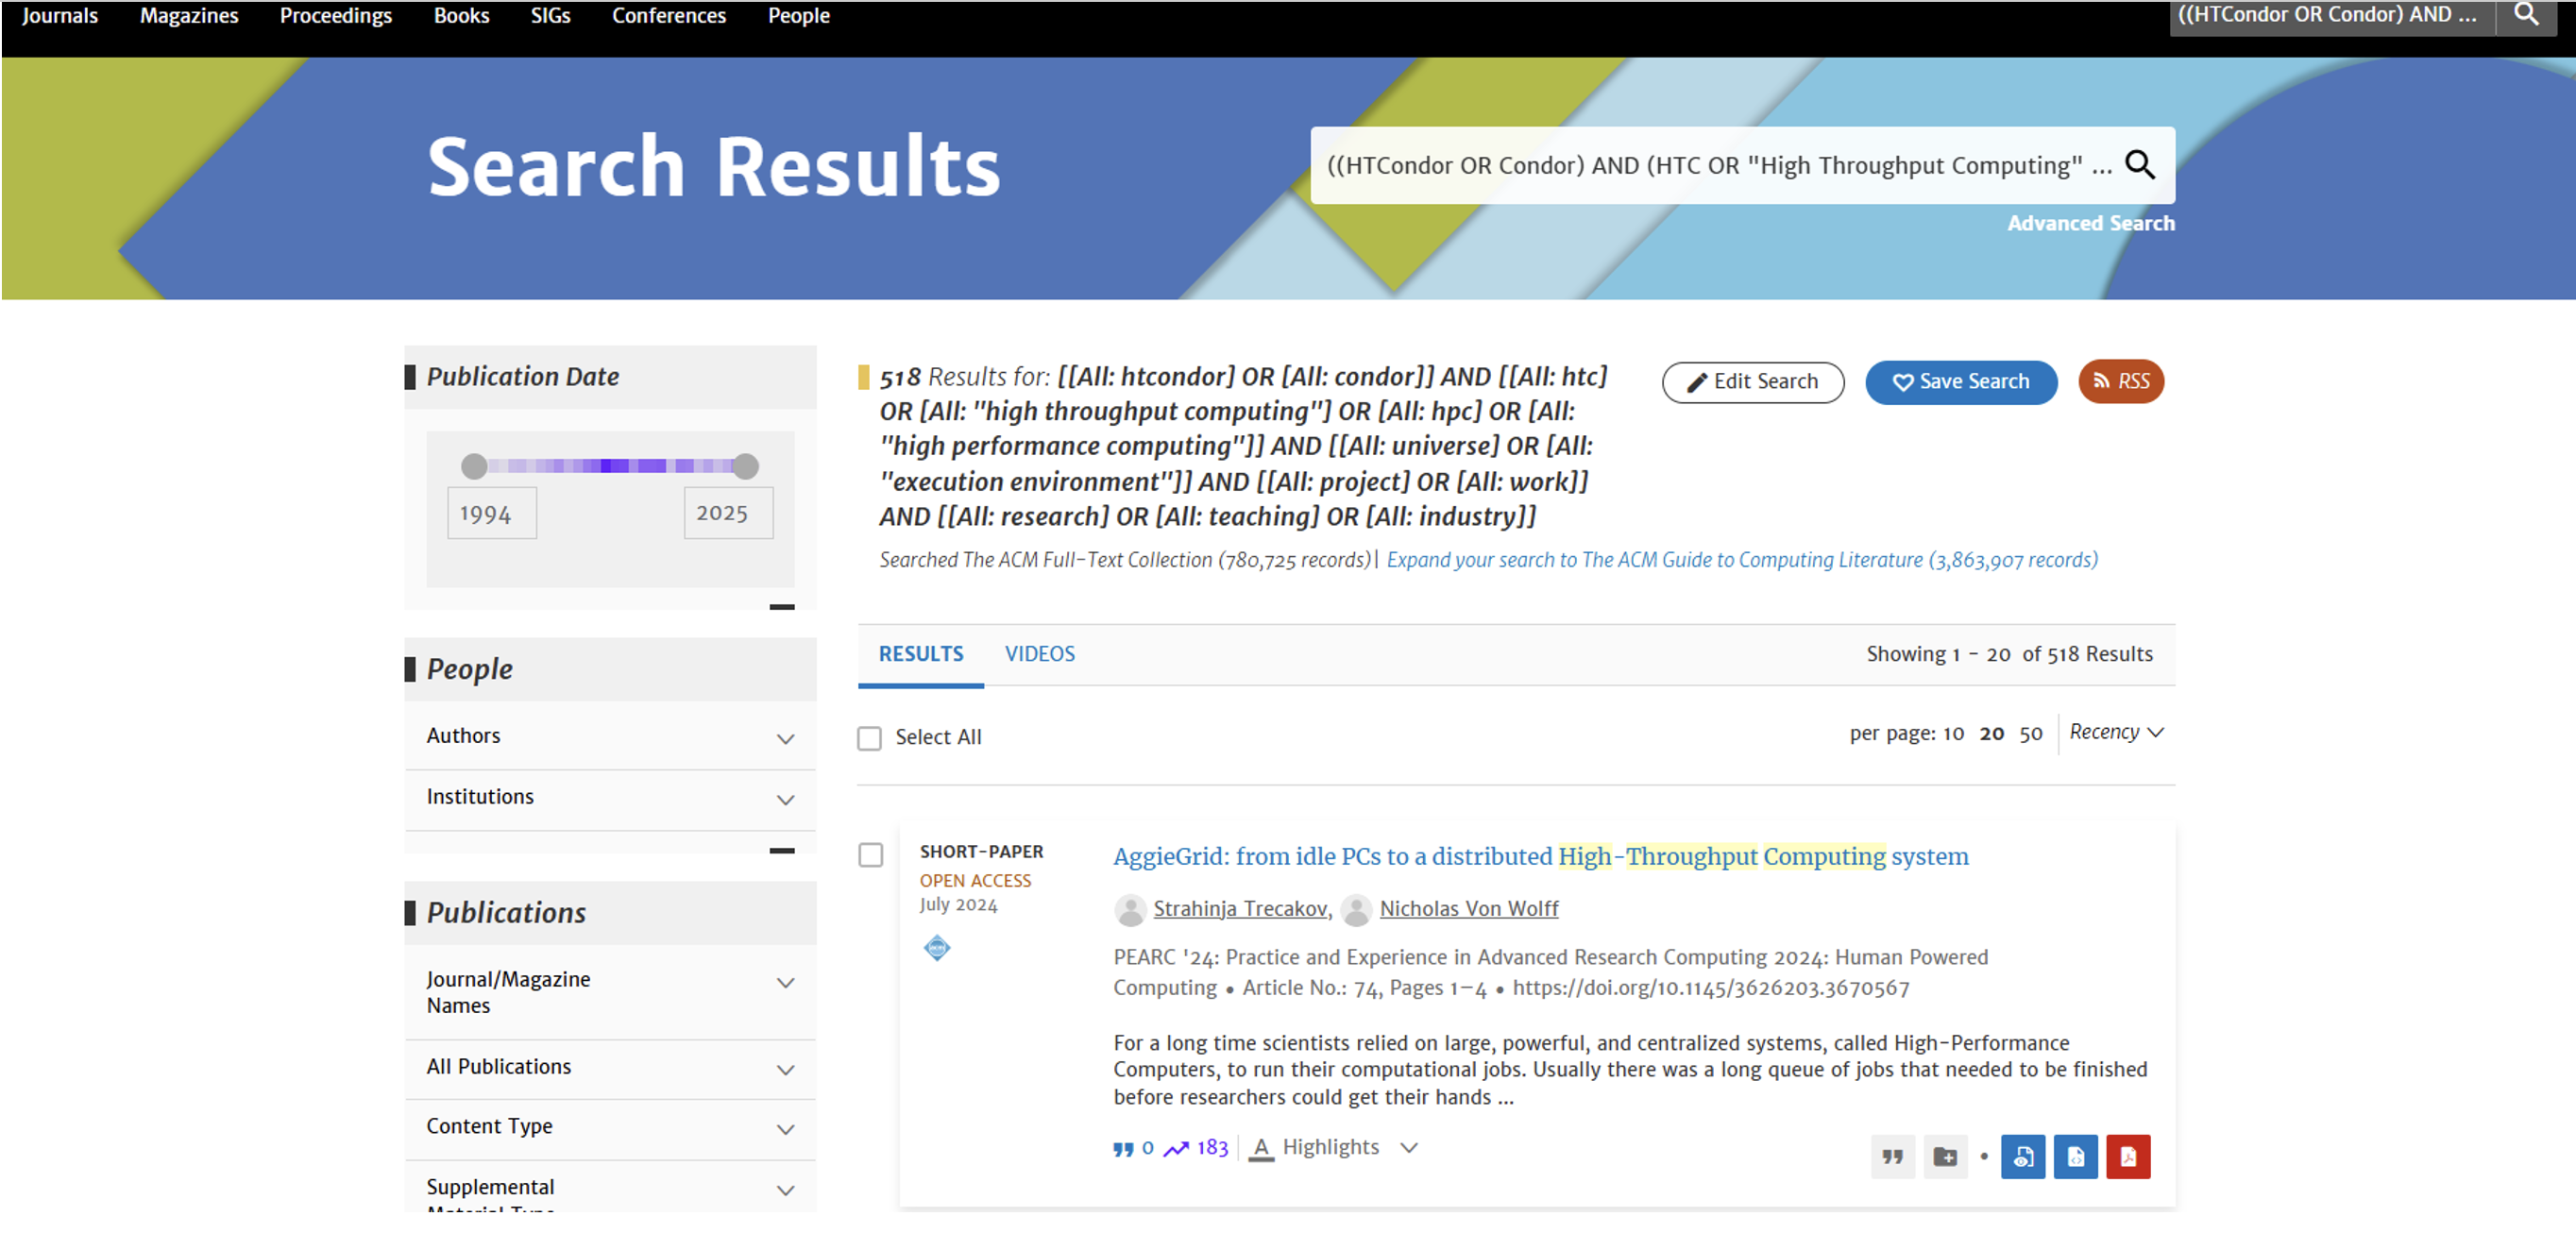
\includegraphics[width=\textwidth,keepaspectratio]{apendices/bases-datos/sin-exclusion/acm.png}
	\caption{Búsqueda de artículos de educación en ACM sin criterios de inclusión/exclusión \\
		Fecha de acceso: 12/03/25 9:13 pm
	}\label{fig:busqueda-acm-no-exclusion}
\end{figure}

\FloatBarrier

\begin{figure}[H]
	\centering
	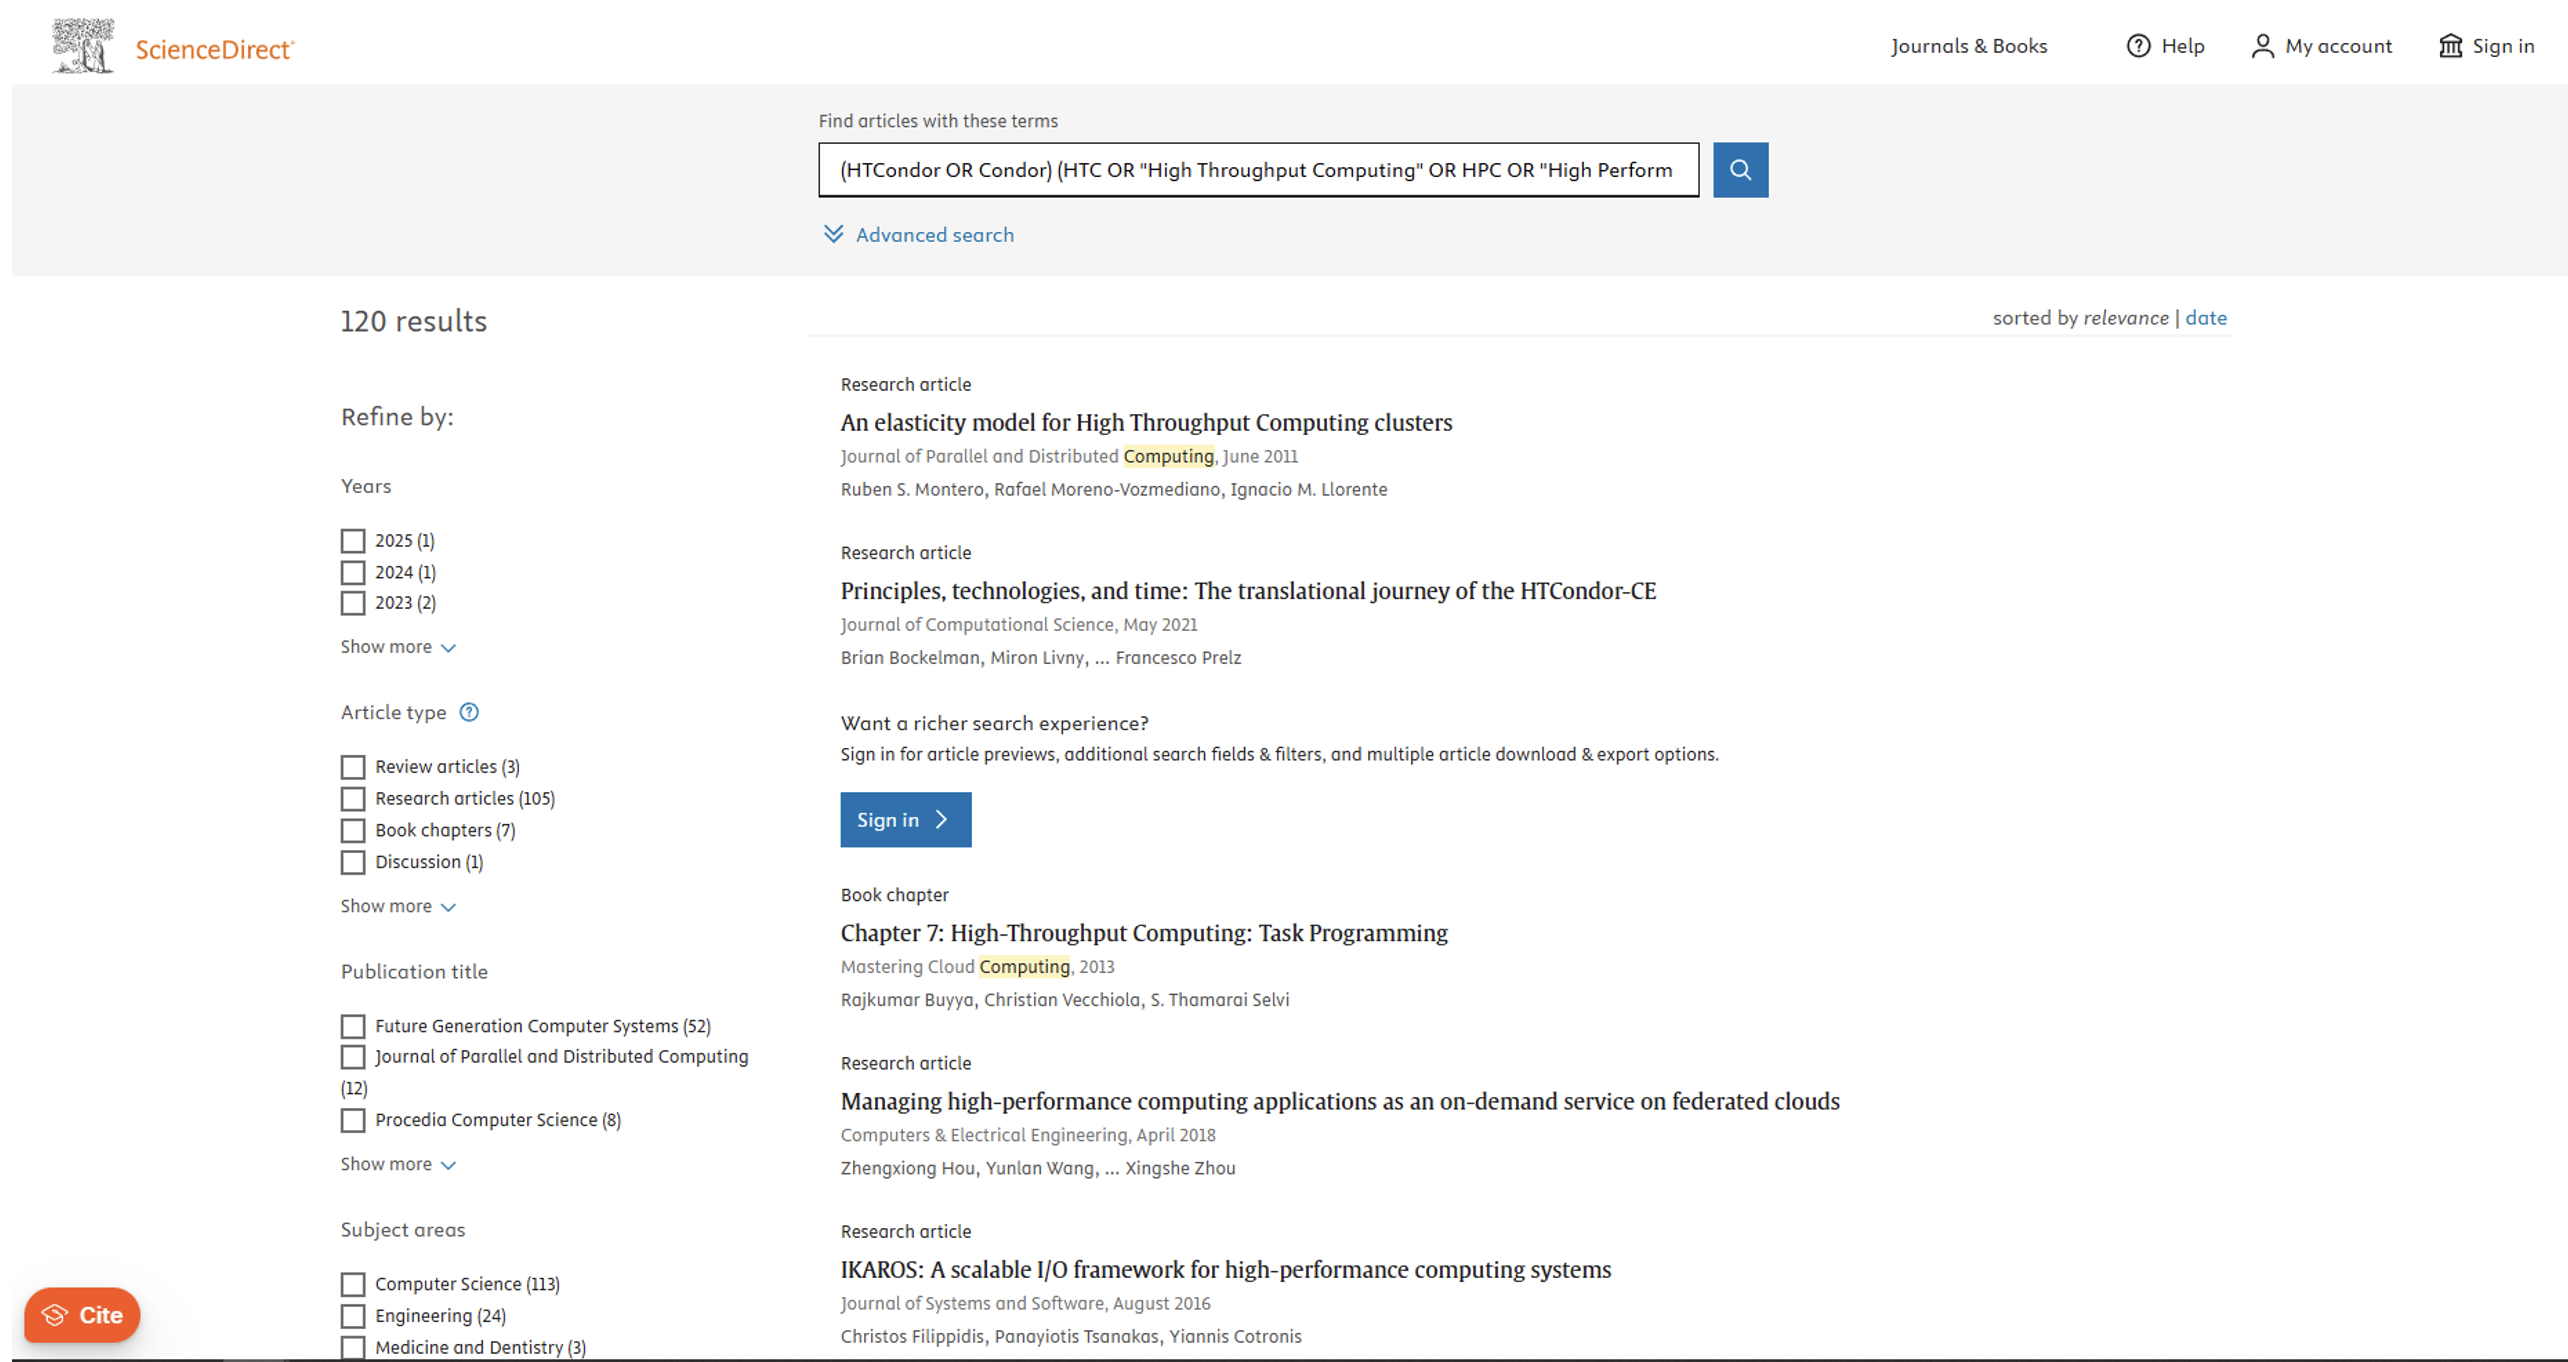
\includegraphics[width=\textwidth,keepaspectratio]{apendices/bases-datos/sin-exclusion/science-direct.png}
	\caption{Búsqueda de artículos de investigación en ACM sin criterios de inclusión/exclusión \\
		Fecha de acceso: 12/03/25 8:23 pm
	}\label{fig:busqueda-science-direct-no-exclusion}
\end{figure}

\begin{figure}[H]
	\centering
	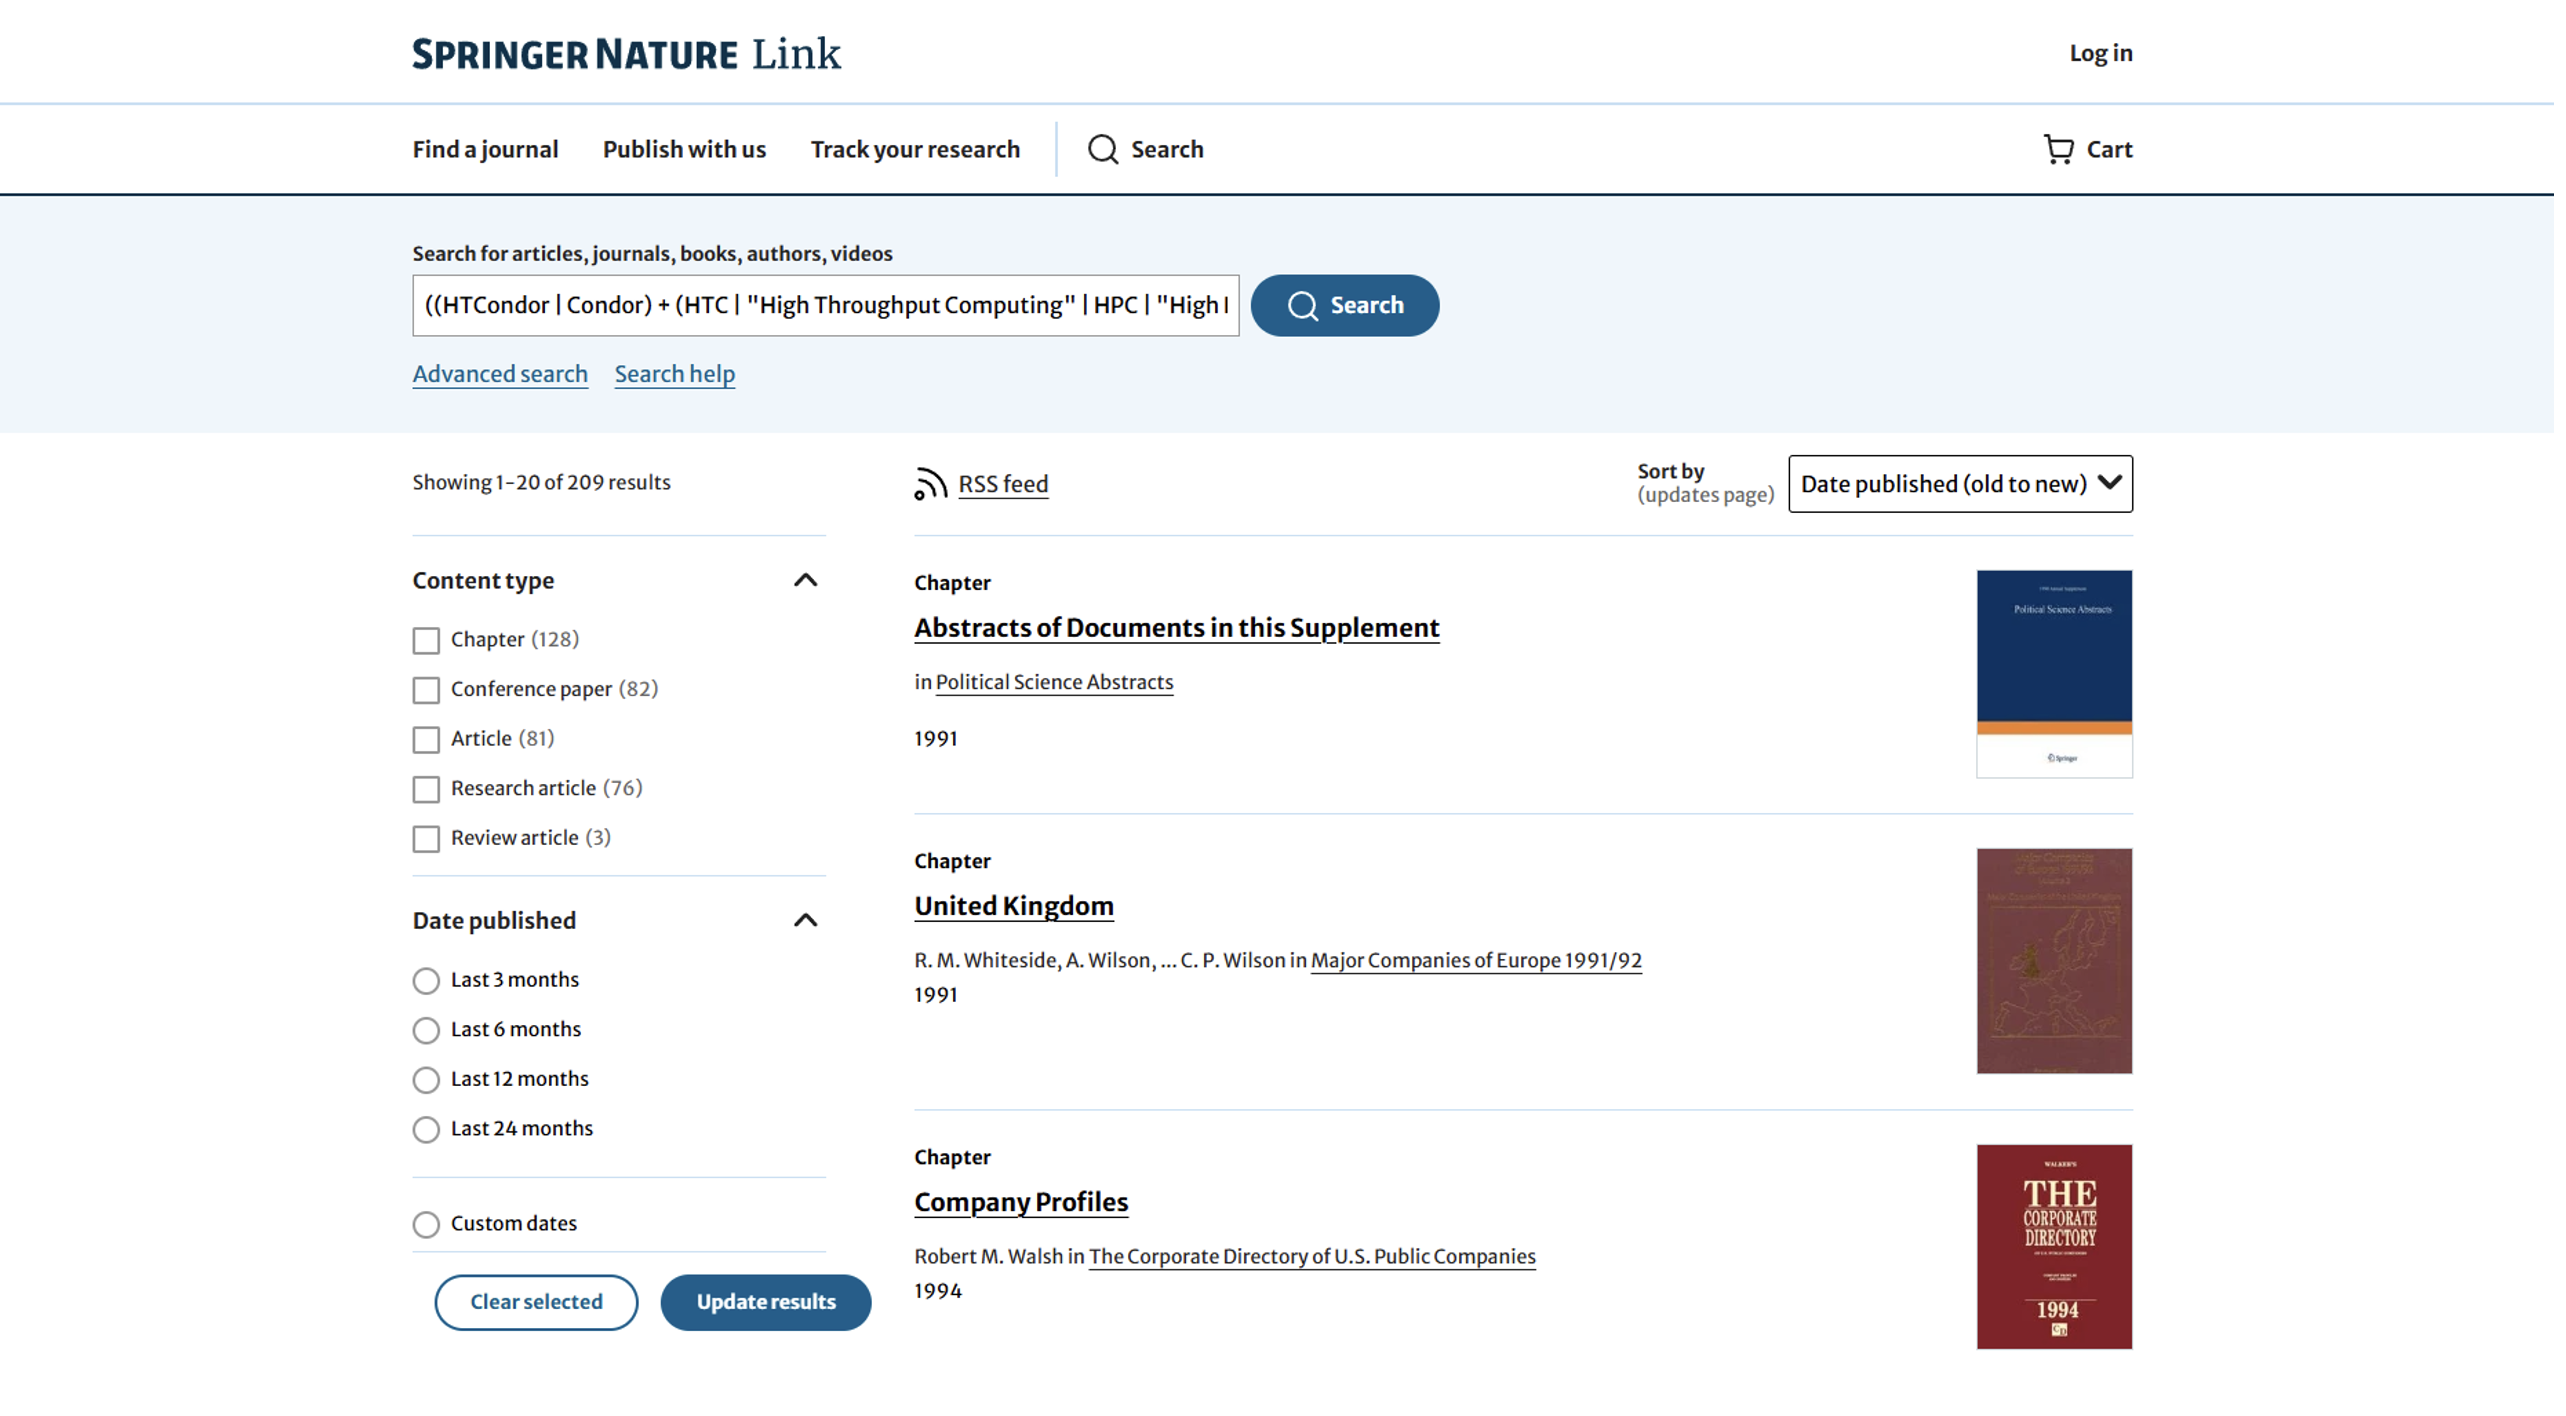
\includegraphics[width=\textwidth,keepaspectratio]{apendices/bases-datos/sin-exclusion/springer.png}
	\caption{Búsqueda de artículos de investigación en ACM sin criterios de inclusión/exclusión \\
		Fecha de acceso: 12/03/25 8:23 pm
	}\label{fig:busqueda-springer-no-exclusion}
\end{figure}


%########## Fin Imagenes %###################


\section{Búsqueda de artículos con criterios de inclusión/exclusión}\label{sec:busqueda-con-criterios}

\begin{figure}[H]
	\centering
	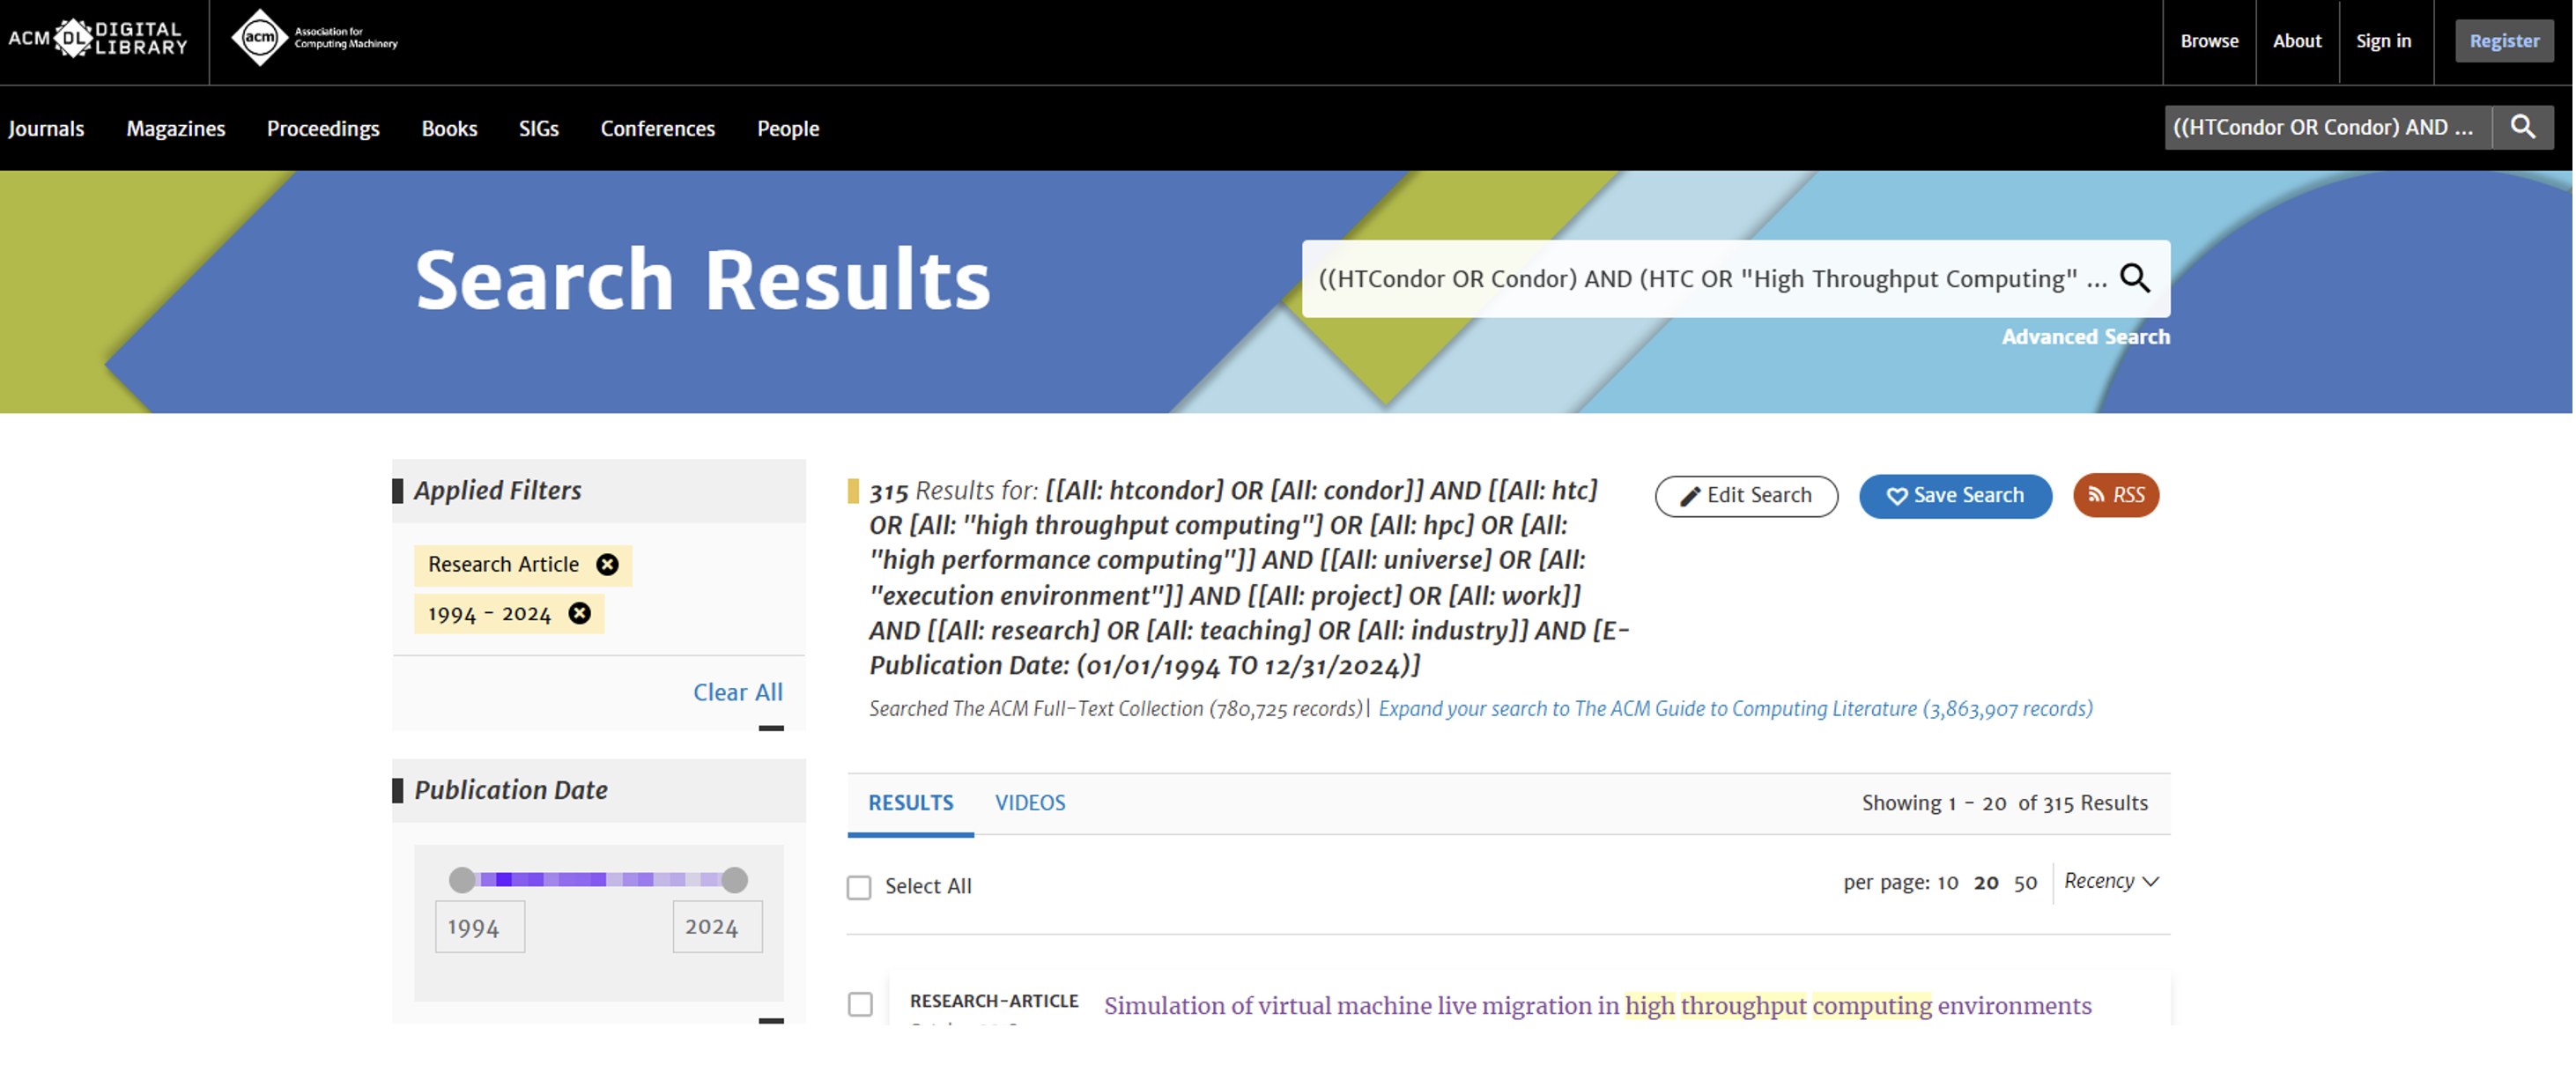
\includegraphics[width=\textwidth,keepaspectratio]{apendices/bases-datos/con-exclusion/acm.png}
	\caption{Búsqueda de artículos de educación en ACM sin criterios de inclusión/exclusión \\
		Fecha de acceso: 12/03/25 9:13 pm
	}\label{fig:busqueda-acm-con-exclusion}
\end{figure}

\FloatBarrier

\begin{figure}[H]
	\centering
	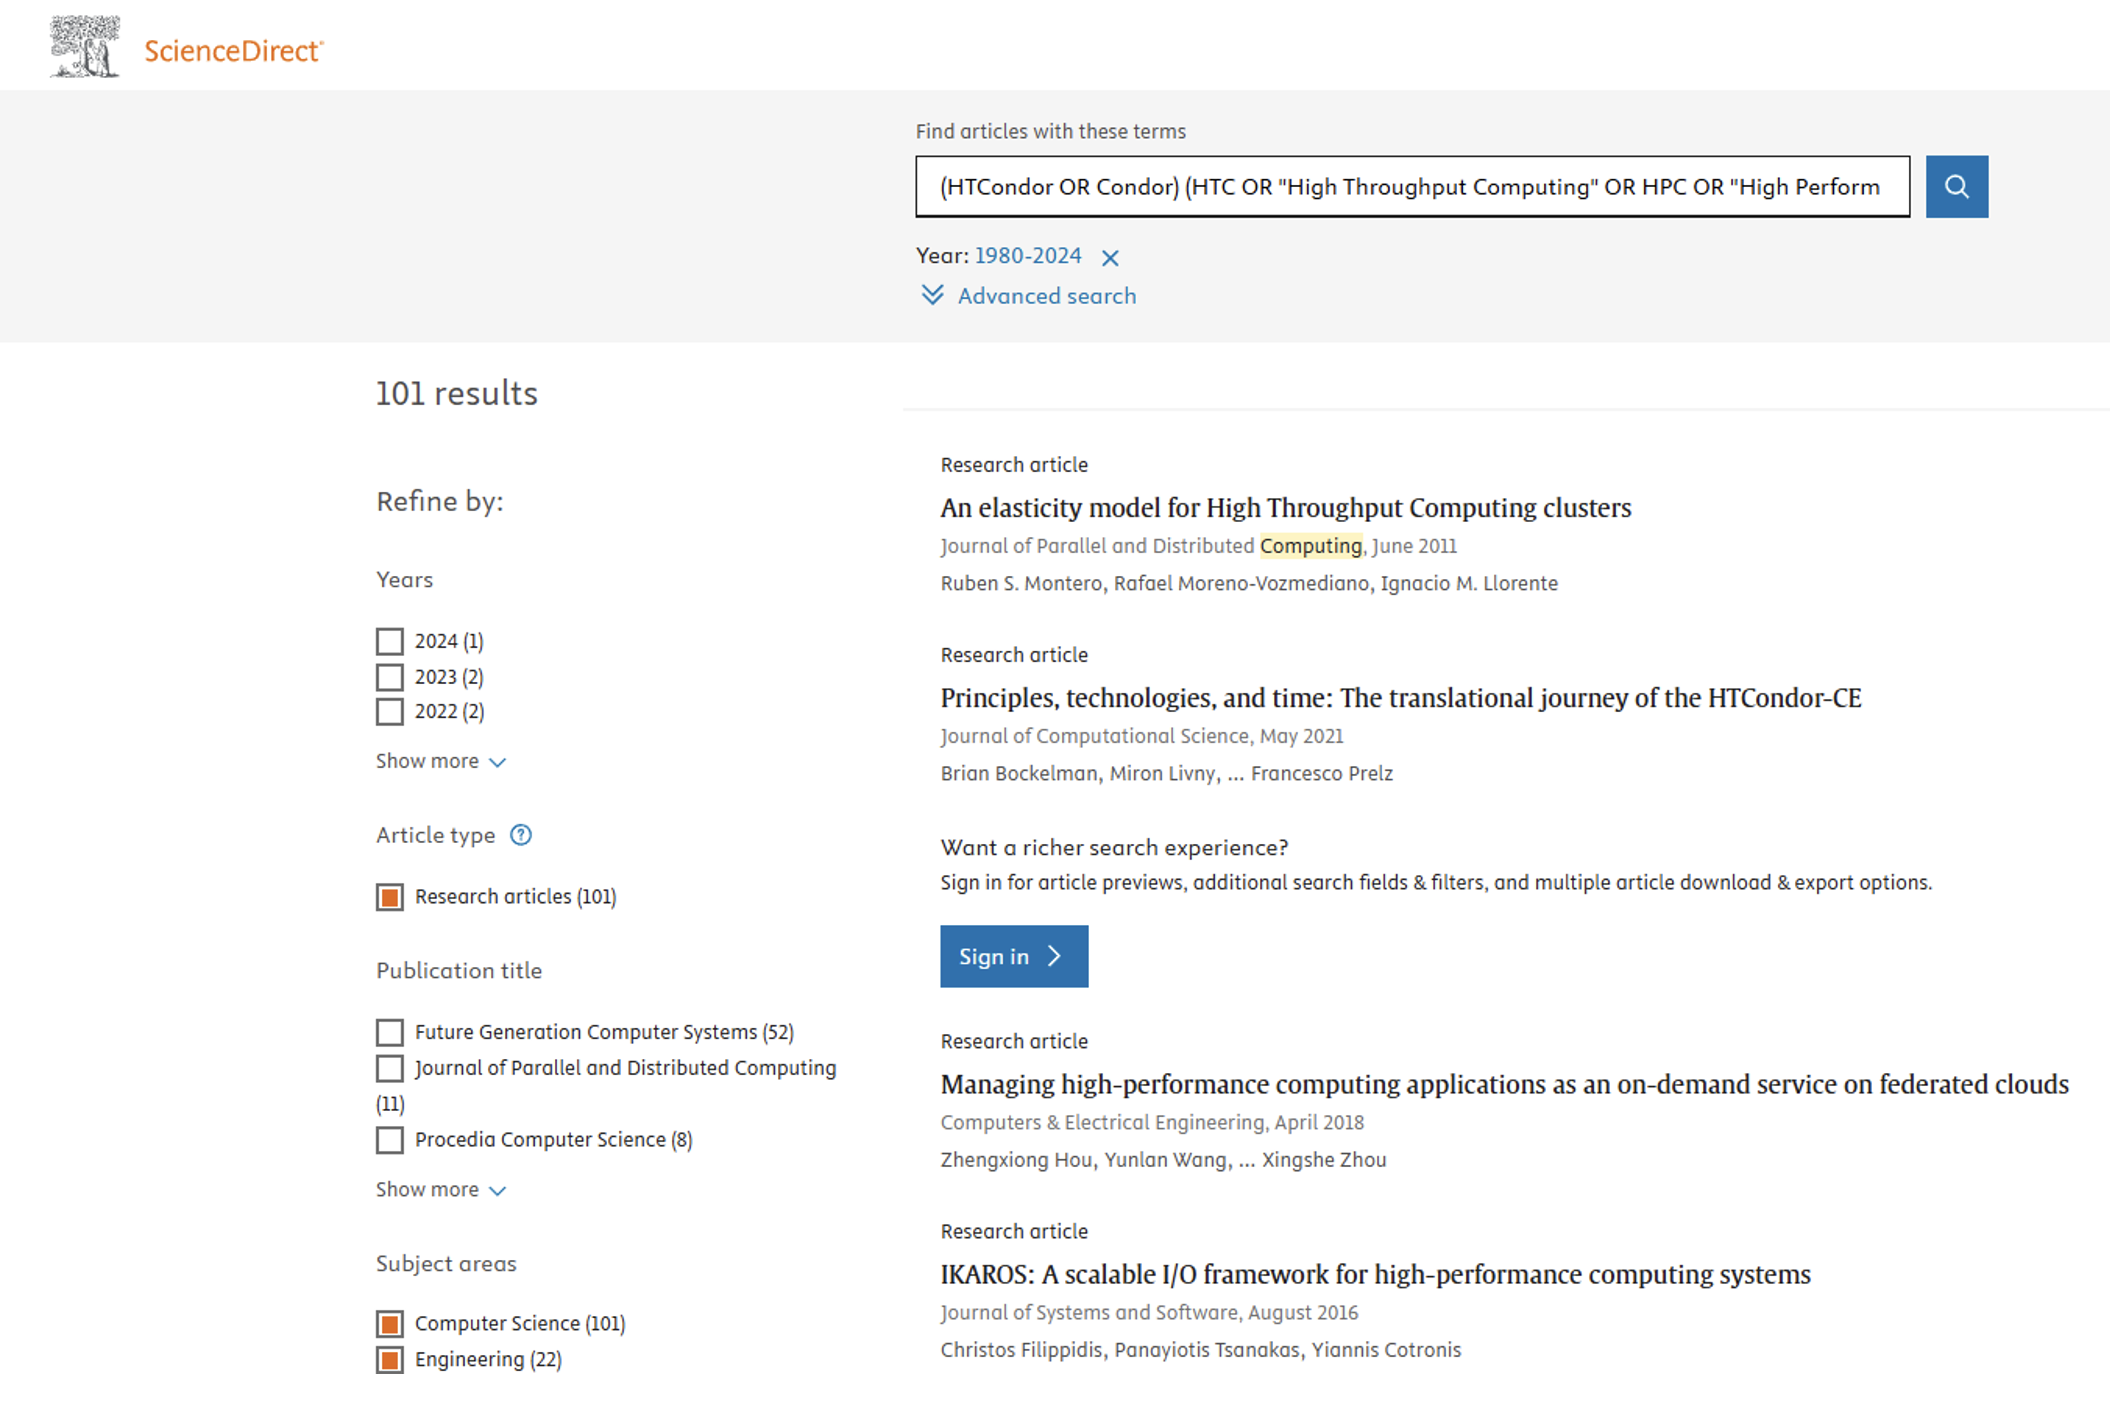
\includegraphics[width=\textwidth,keepaspectratio]{apendices/bases-datos/con-exclusion/science-direct.png}
	\caption{Búsqueda de artículos de investigación en ACM sin criterios de inclusión/exclusión \\
		Fecha de acceso: 12/03/25 8:23 pm
	}\label{fig:busqueda-science-direct-con-exclusion}
\end{figure}

\begin{figure}[H]
	\centering
	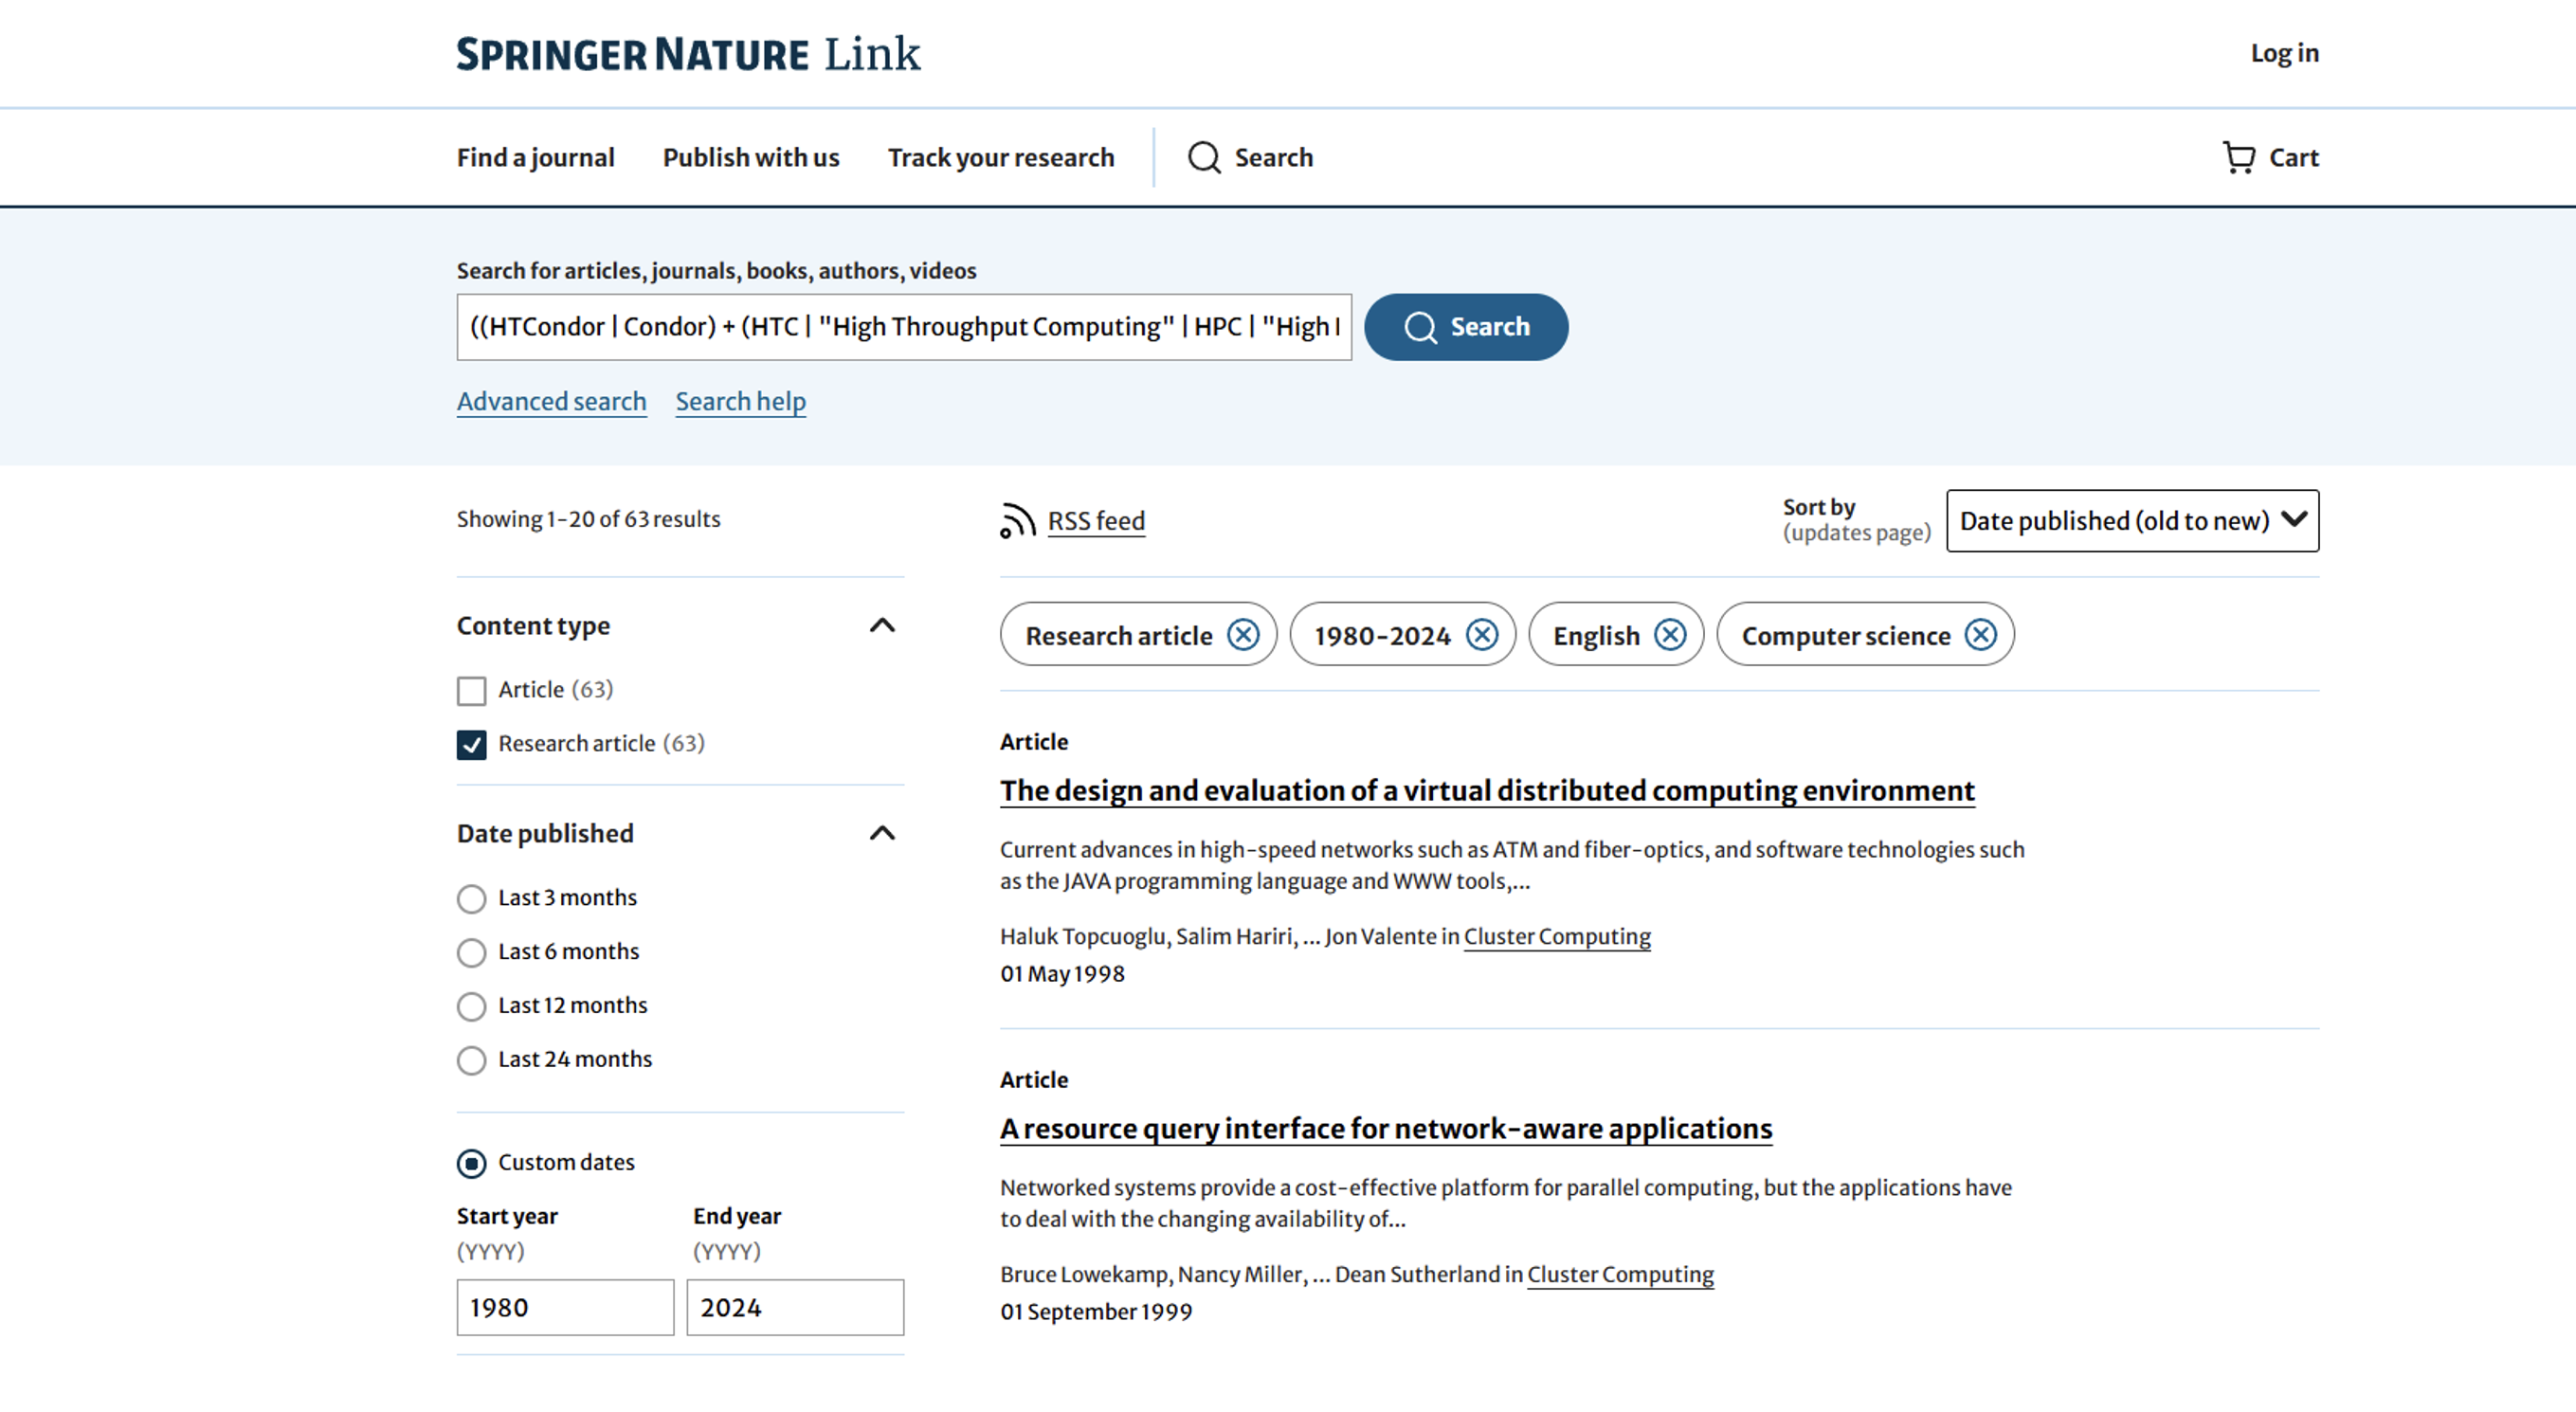
\includegraphics[width=\textwidth,keepaspectratio]{apendices/bases-datos/con-exclusion/springer.png}
	\caption{Búsqueda de artículos de investigación en ACM sin criterios de inclusión/exclusión \\
		Fecha de acceso: 12/03/25 8:23 pm
	}\label{fig:busqueda-springer-con-exclusion}
\end{figure}



%
%\FloatBarrier\chapter{Plantilla del análisis DAR}
%\section{Plantilla análisis DAR}
%
%\begin{figure}[H]
%	\centering
%	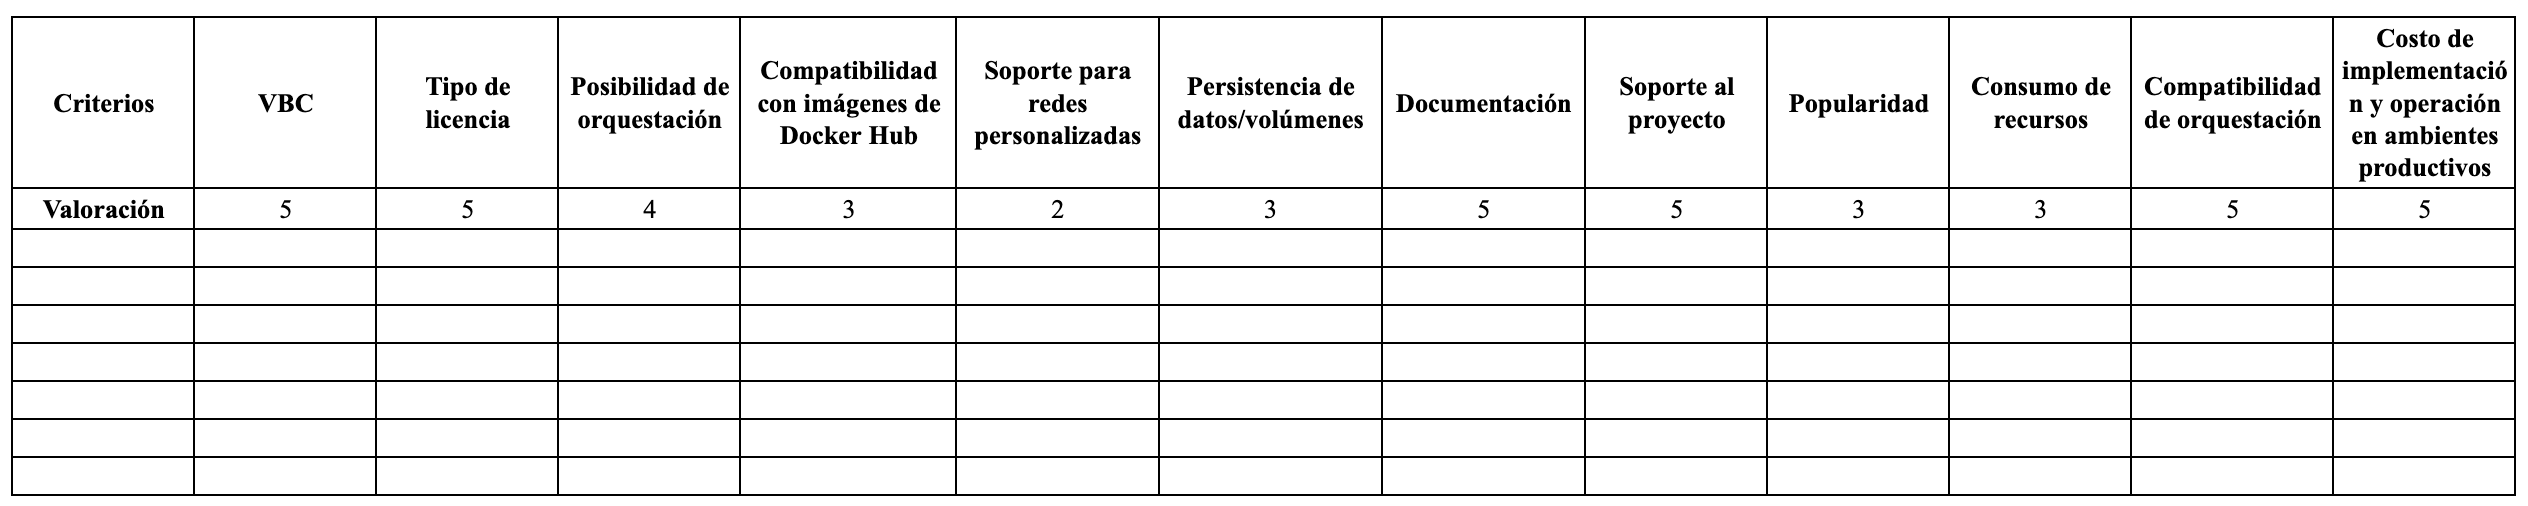
\includegraphics[width=\textwidth,height=0.85\textheight,keepaspectratio]{apendices/plantilla-DAR.png}
%	\caption{Plantilla del análisis DAR}\label{fig:tabla-plantilla-dar}
%\end{figure}
%\FloatBarrier\chapter{Eventos de difusión}
%\section{Seminario GRID 2024-II}
%
%
%\section{Seminario GRID 2025-I}
%
%\section{ACOFI 2025}
%
%En esta sección se presenta la ponencia presentada en el congreso ACOFI 2025 como resultado de la investigación desarrollada en este trabajo.
%
%\subsection{Páginas de la ponencia ACOFI}
%
%% Página 1
%\begin{figure}[H]
%	\centering
%	\begin{tcolorbox}[
%			colback=white,
%			colframe=gray!50,
%			boxrule=1pt,
%			arc=2pt,
%			boxsep=5pt,
%			left=3pt,
%			right=3pt,
%			top=3pt,
%			bottom=3pt,
%			drop shadow
%		]
%		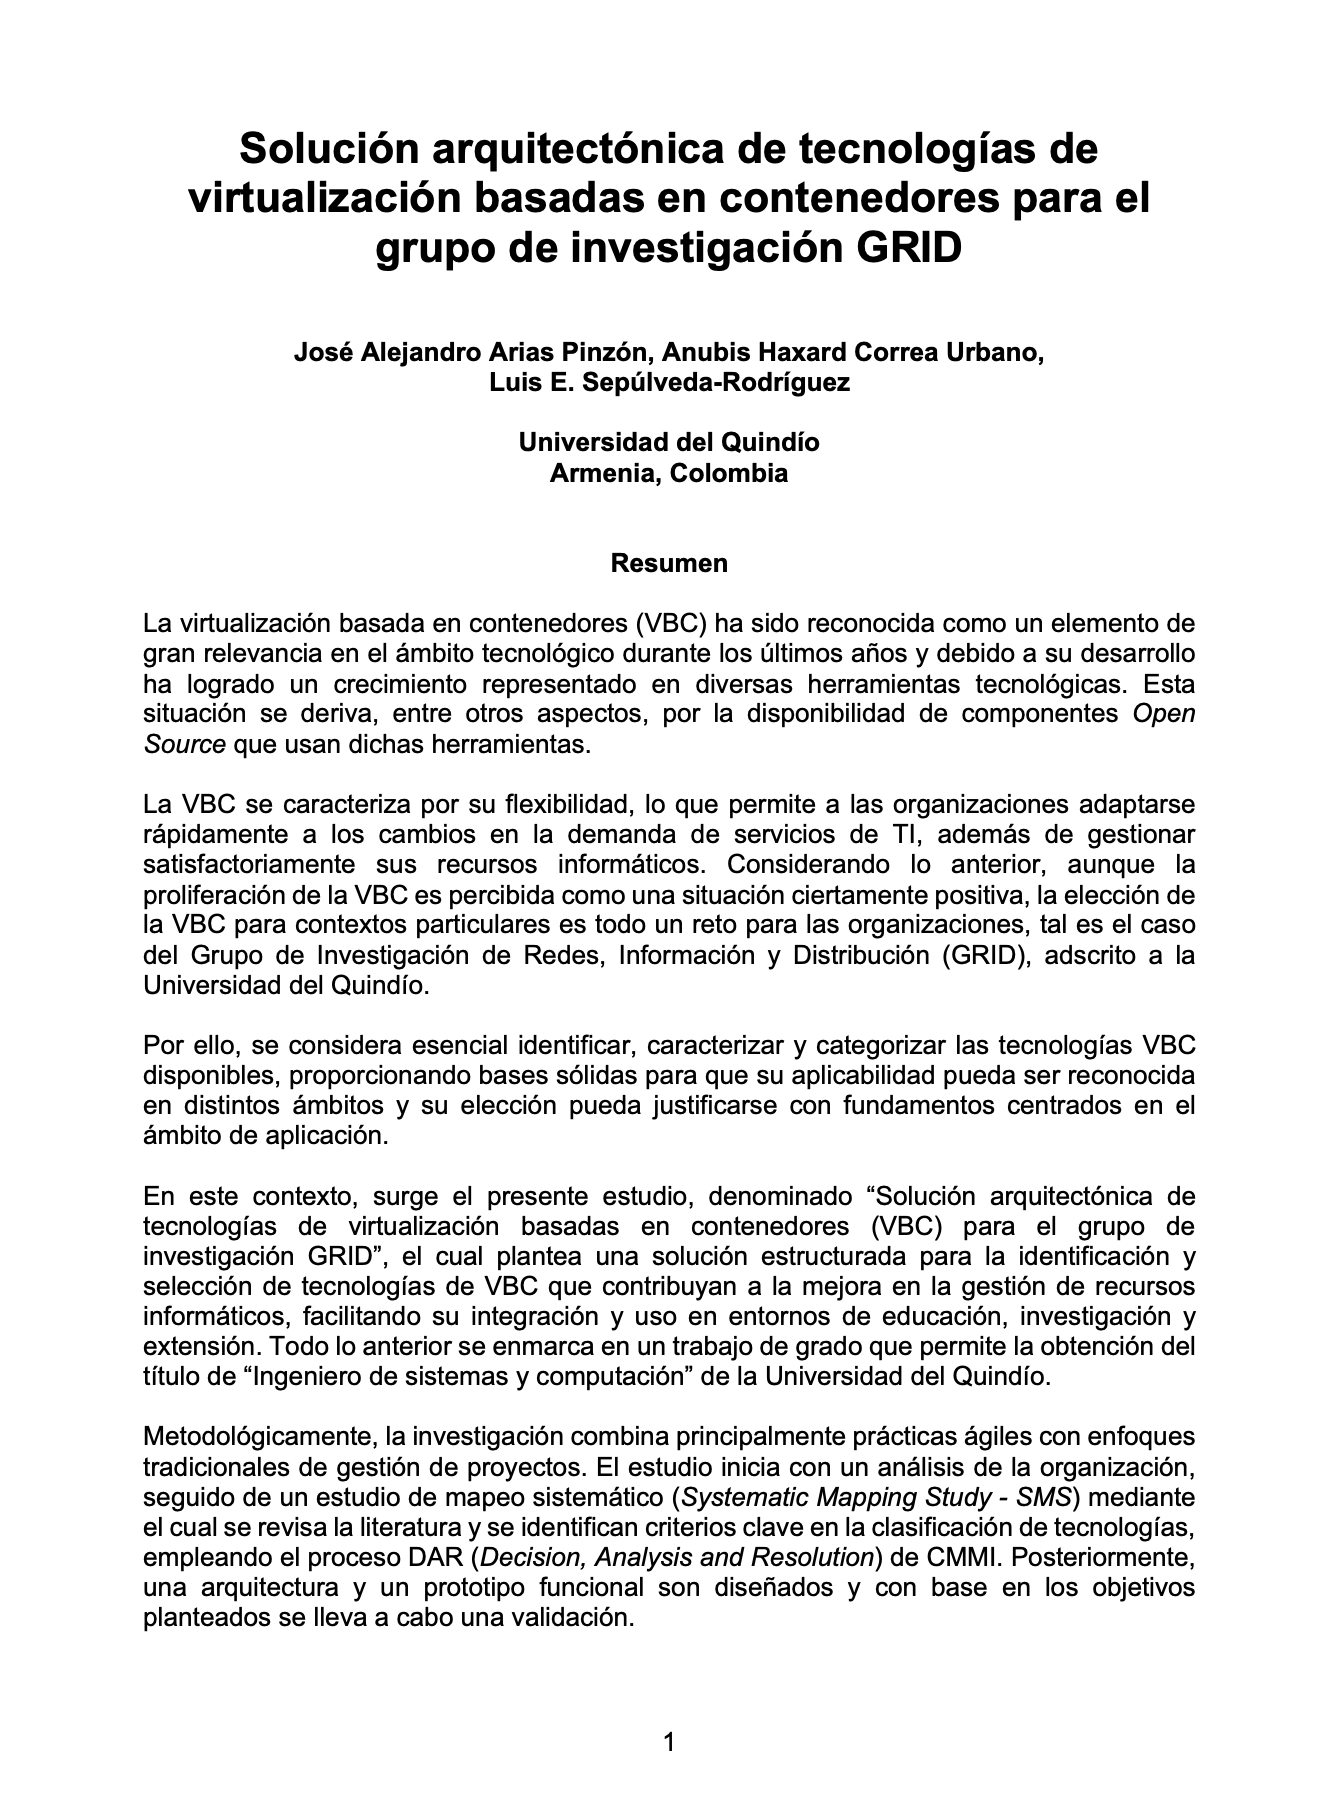
\includegraphics[width=0.95\textwidth,keepaspectratio]{apendices/ACOFI/pagina_1.png}
%	\end{tcolorbox}
%	\caption{Ponencia ACOFI --- Página 1}\label{fig:acofi-pagina-1}
%\end{figure}
%\FloatBarrier% Página 2
%\begin{figure}[H]
%	\centering
%	\begin{tcolorbox}[
%			colback=white,
%			colframe=gray!50,
%			boxrule=1pt,
%			arc=2pt,
%			boxsep=5pt,
%			left=3pt,
%			right=3pt,
%			top=3pt,
%			bottom=3pt,
%			drop shadow
%		]
%		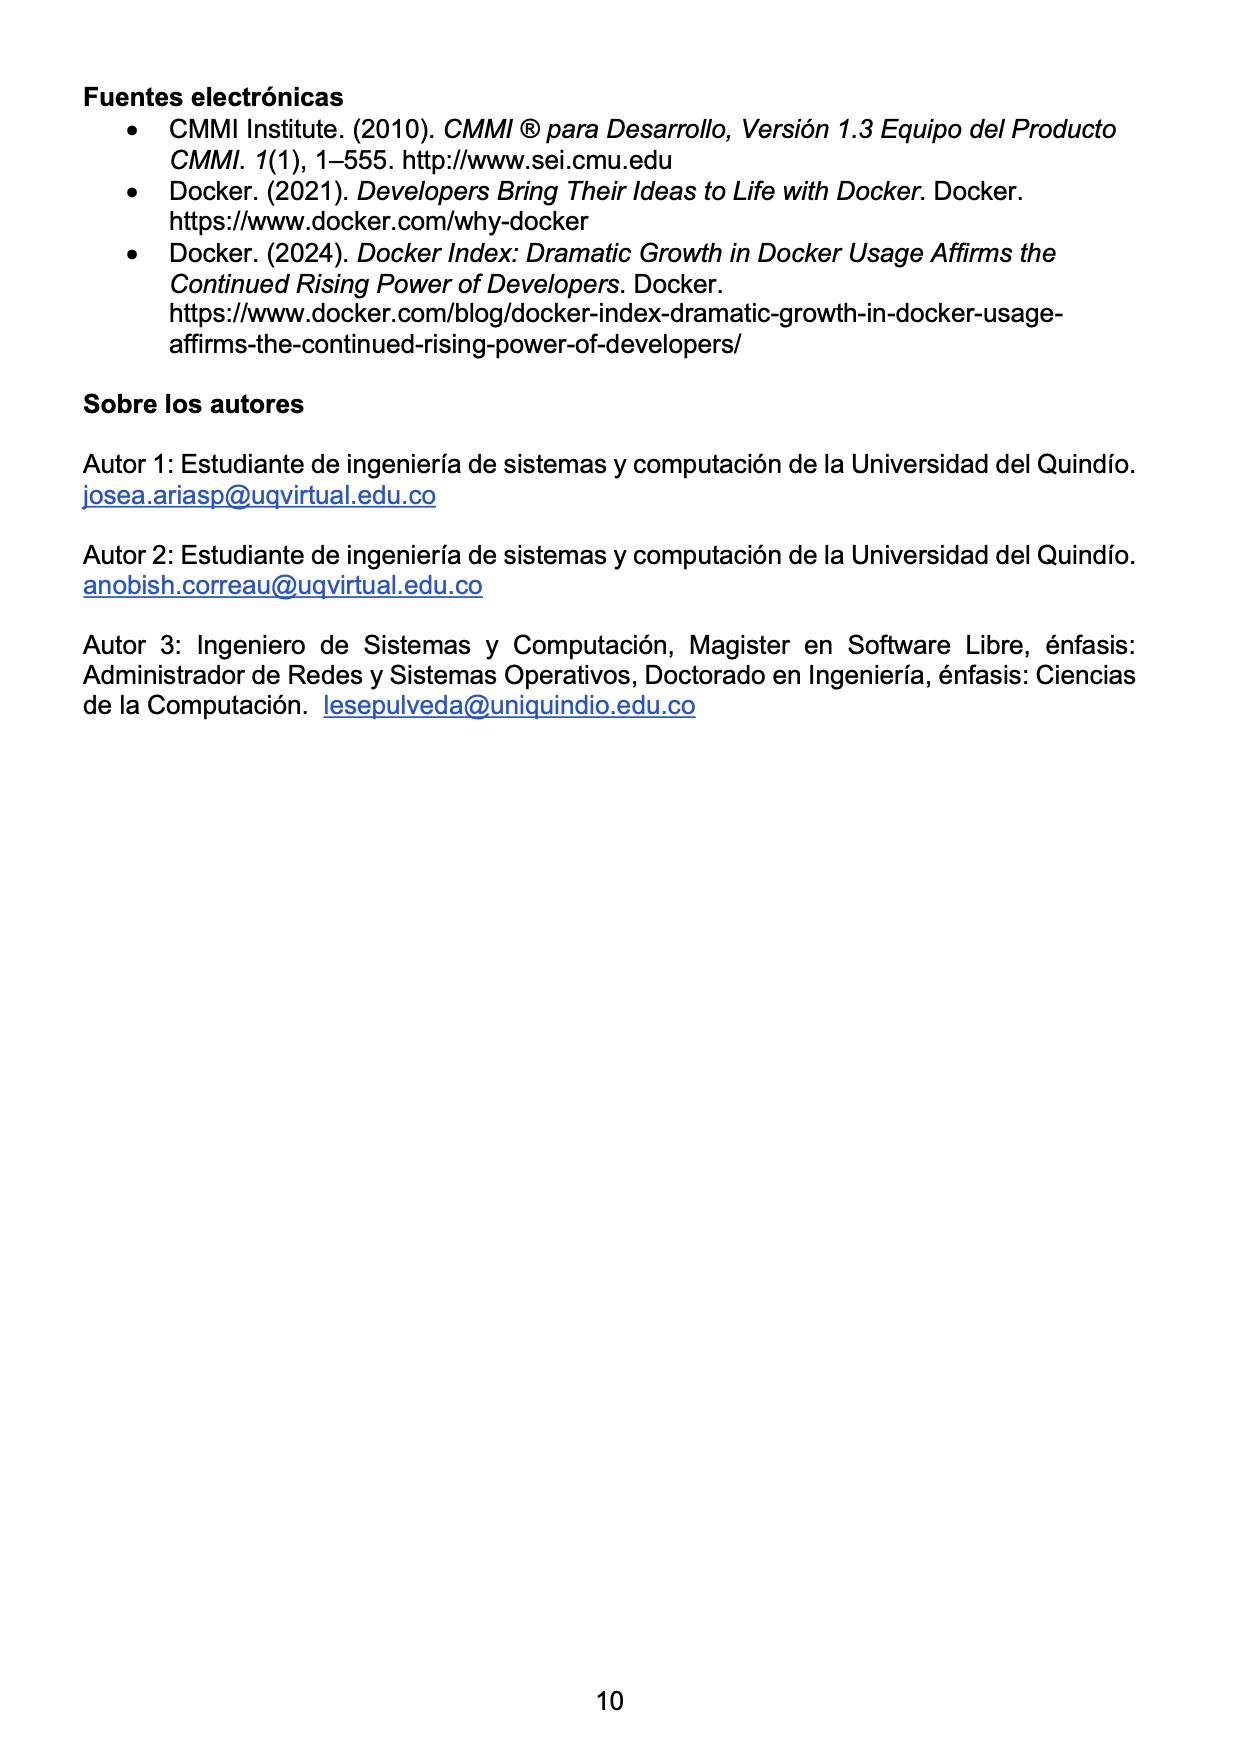
\includegraphics[width=0.95\textwidth,keepaspectratio]{apendices/ACOFI/pagina_2.png}
%	\end{tcolorbox}
%	\caption{Ponencia ACOFI --- Página 2}\label{fig:acofi-pagina-2}
%\end{figure}
%\FloatBarrier% Página 3
%\begin{figure}[H]
%	\centering
%	\begin{tcolorbox}[
%			colback=white,
%			colframe=gray!50,
%			boxrule=1pt,
%			arc=2pt,
%			boxsep=5pt,
%			left=3pt,
%			right=3pt,
%			top=3pt,
%			bottom=3pt,
%			drop shadow
%		]
%		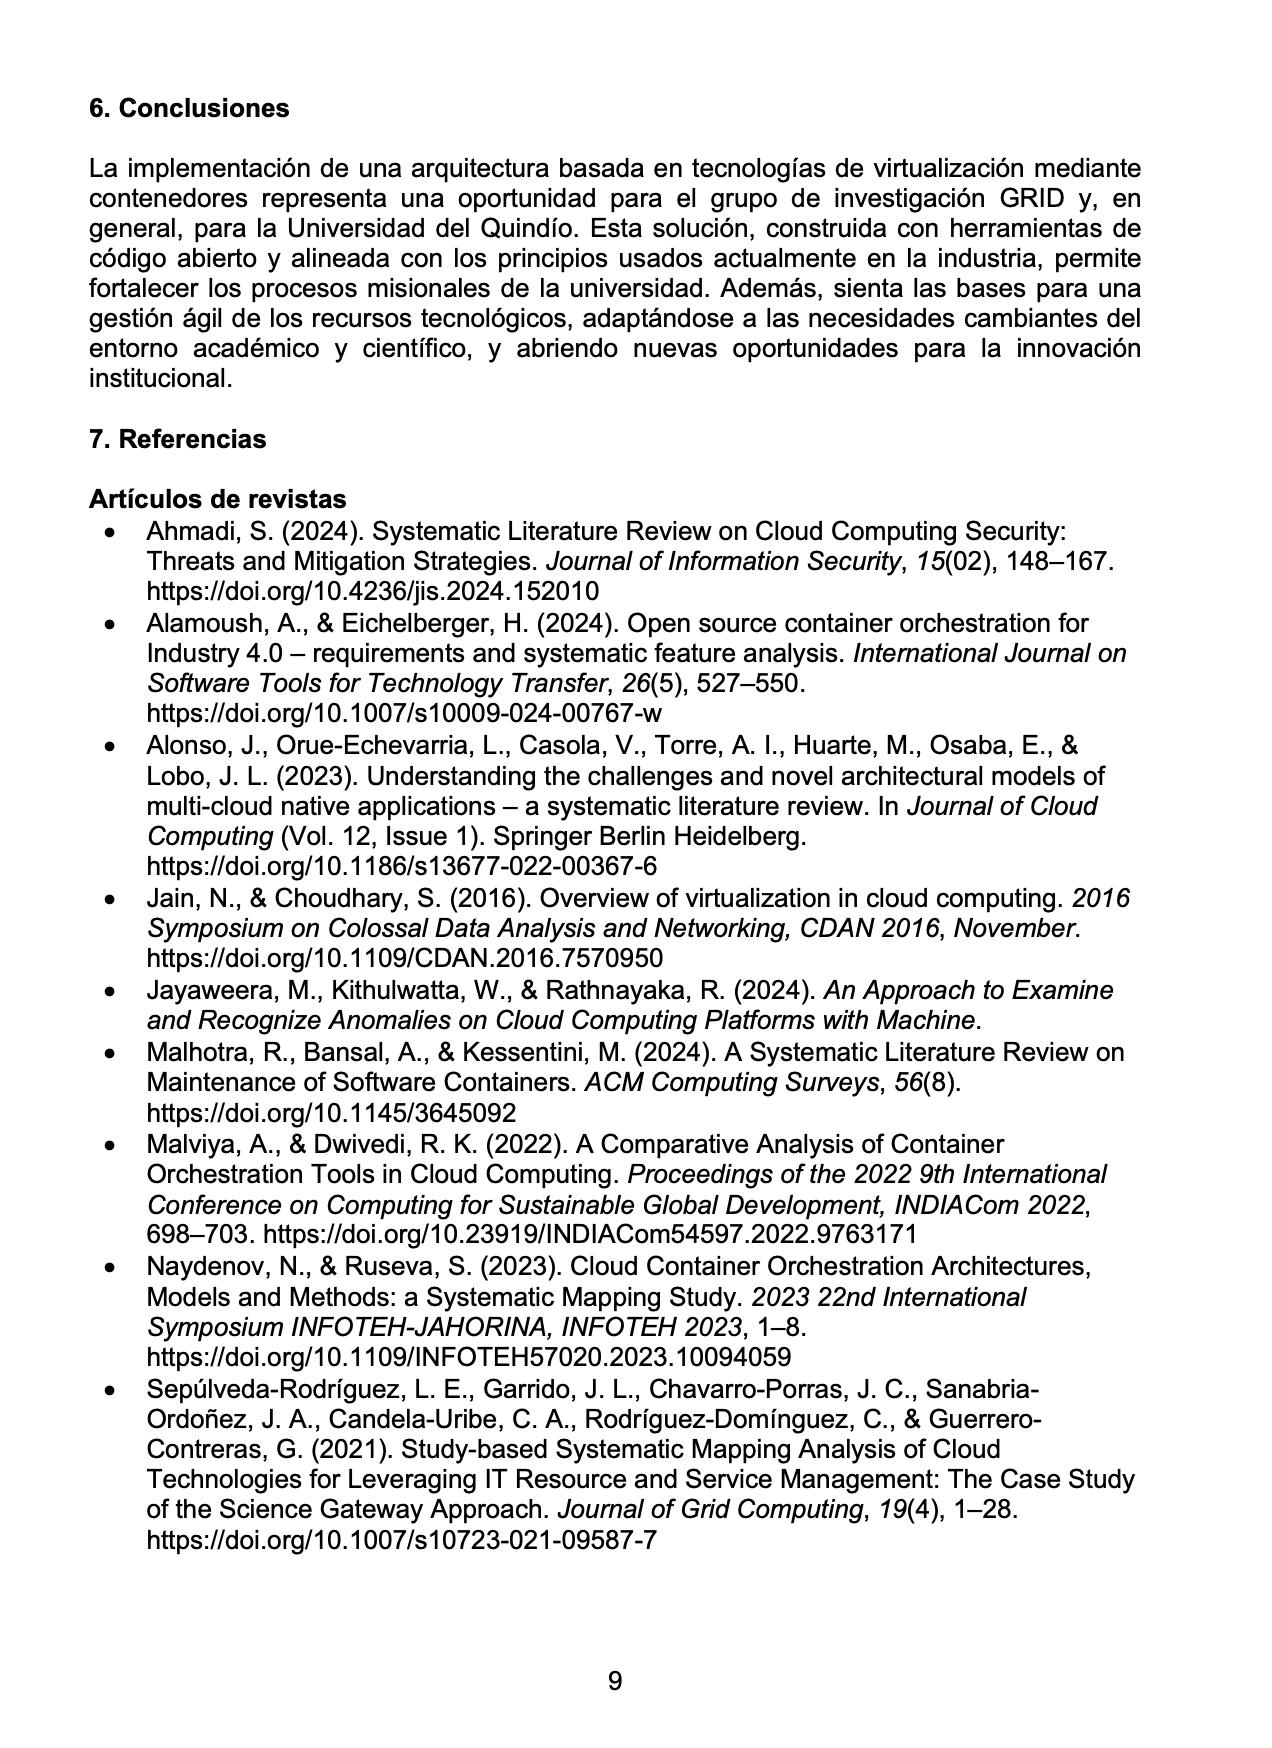
\includegraphics[width=0.95\textwidth,keepaspectratio]{apendices/ACOFI/pagina_3.png}
%	\end{tcolorbox}
%	\caption{Ponencia ACOFI --- Página 3}\label{fig:acofi-pagina-3}
%\end{figure}
%\FloatBarrier% Página 4
%\begin{figure}[H]
%	\centering
%	\begin{tcolorbox}[
%			colback=white,
%			colframe=gray!50,
%			boxrule=1pt,
%			arc=2pt,
%			boxsep=5pt,
%			left=3pt,
%			right=3pt,
%			top=3pt,
%			bottom=3pt,
%			drop shadow
%		]
%		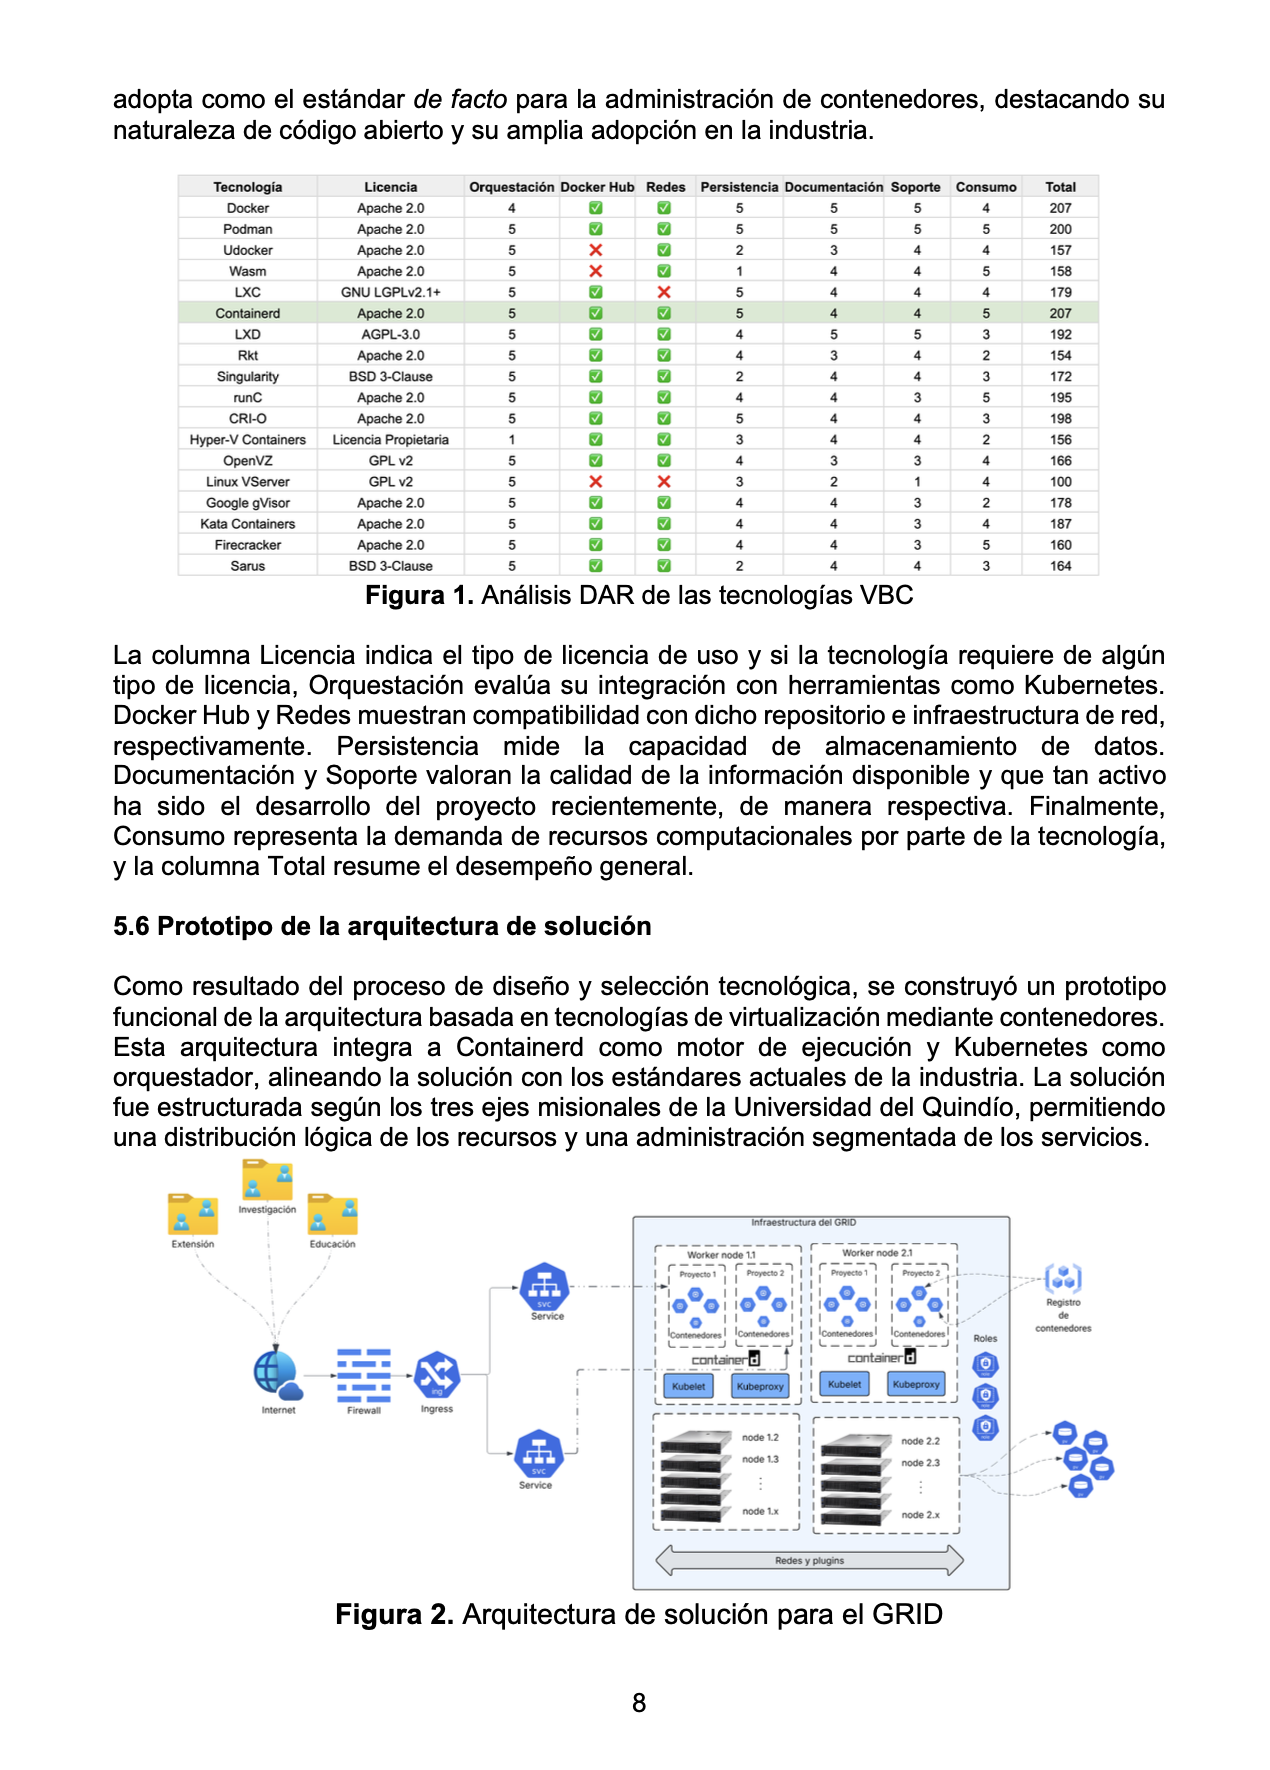
\includegraphics[width=0.95\textwidth,keepaspectratio]{apendices/ACOFI/pagina_4.png}
%	\end{tcolorbox}
%	\caption{Ponencia ACOFI --- Página 4}\label{fig:acofi-pagina-4}
%\end{figure}
%\FloatBarrier% Página 5
%\begin{figure}[H]
%	\centering
%	\begin{tcolorbox}[
%			colback=white,
%			colframe=gray!50,
%			boxrule=1pt,
%			arc=2pt,
%			boxsep=5pt,
%			left=3pt,
%			right=3pt,
%			top=3pt,
%			bottom=3pt,
%			drop shadow
%		]
%		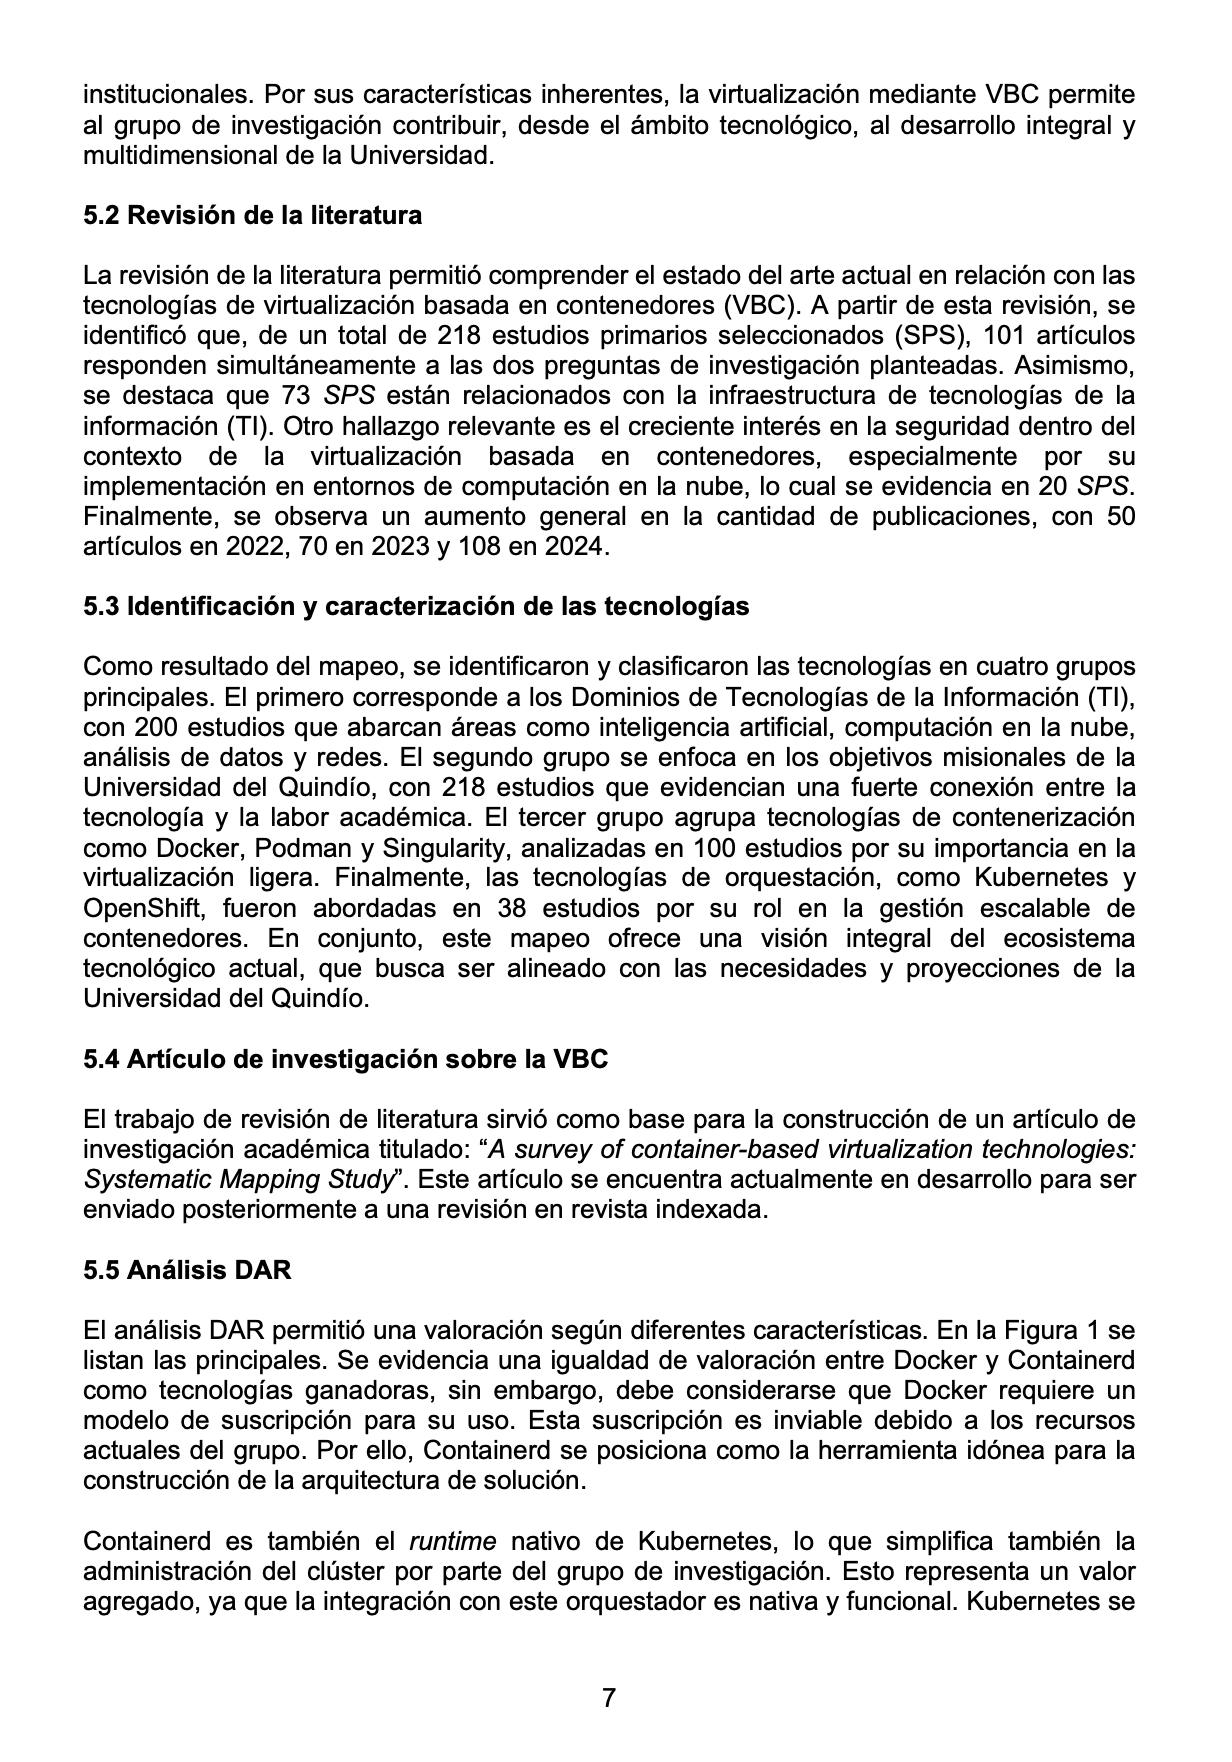
\includegraphics[width=0.95\textwidth,keepaspectratio]{apendices/ACOFI/pagina_5.png}
%	\end{tcolorbox}
%	\caption{Ponencia ACOFI --- Página 5}\label{fig:acofi-pagina-5}
%\end{figure}
%\FloatBarrier% Página 6
%\begin{figure}[H]
%	\centering
%	\begin{tcolorbox}[
%			colback=white,
%			colframe=gray!50,
%			boxrule=1pt,
%			arc=2pt,
%			boxsep=5pt,
%			left=3pt,
%			right=3pt,
%			top=3pt,
%			bottom=3pt,
%			drop shadow
%		]
%		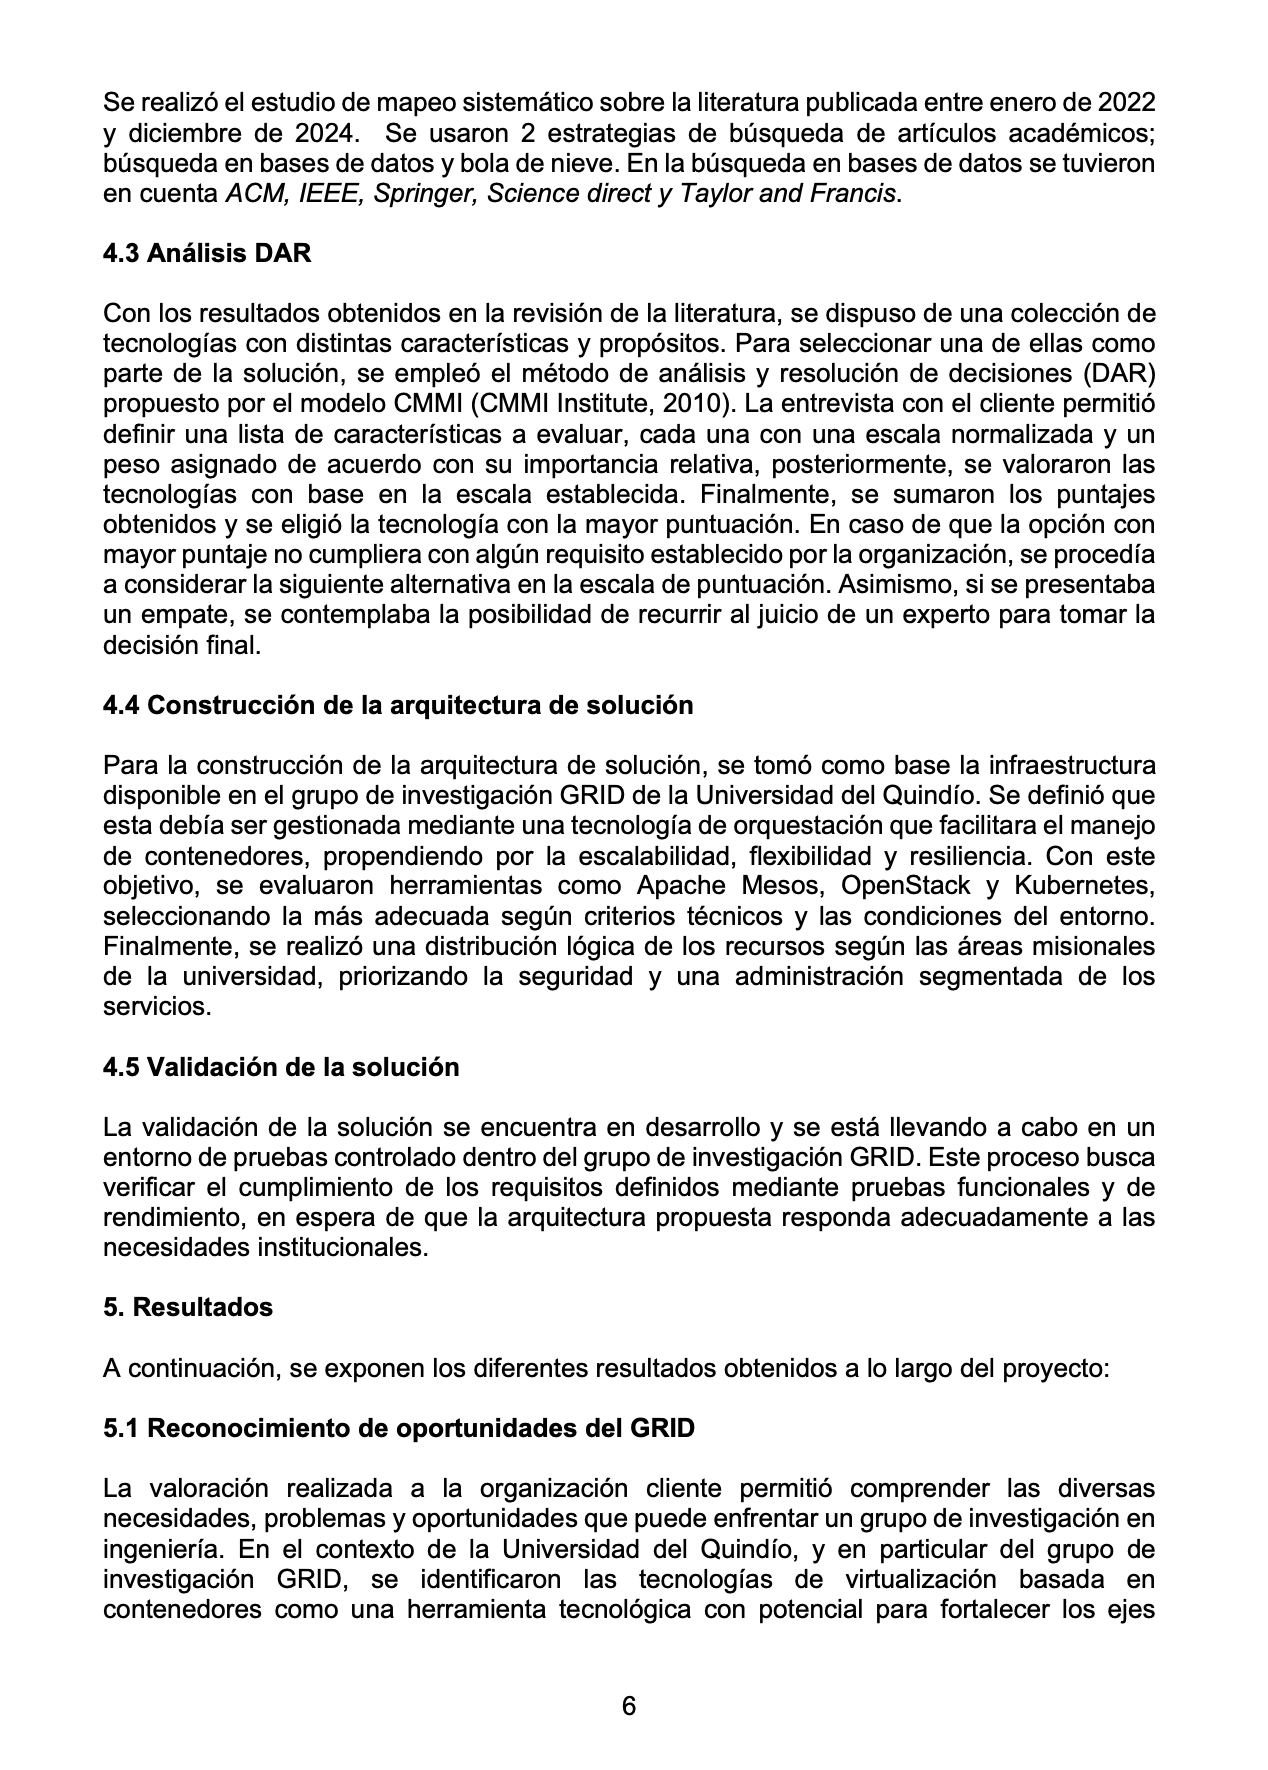
\includegraphics[width=0.95\textwidth,keepaspectratio]{apendices/ACOFI/pagina_6.png}
%	\end{tcolorbox}
%	\caption{Ponencia ACOFI --- Página 6}\label{fig:acofi-pagina-6}
%\end{figure}
%\FloatBarrier% Página 7
%\begin{figure}[H]
%	\centering
%	\begin{tcolorbox}[
%			colback=white,
%			colframe=gray!50,
%			boxrule=1pt,
%			arc=2pt,
%			boxsep=5pt,
%			left=3pt,
%			right=3pt,
%			top=3pt,
%			bottom=3pt,
%			drop shadow
%		]
%		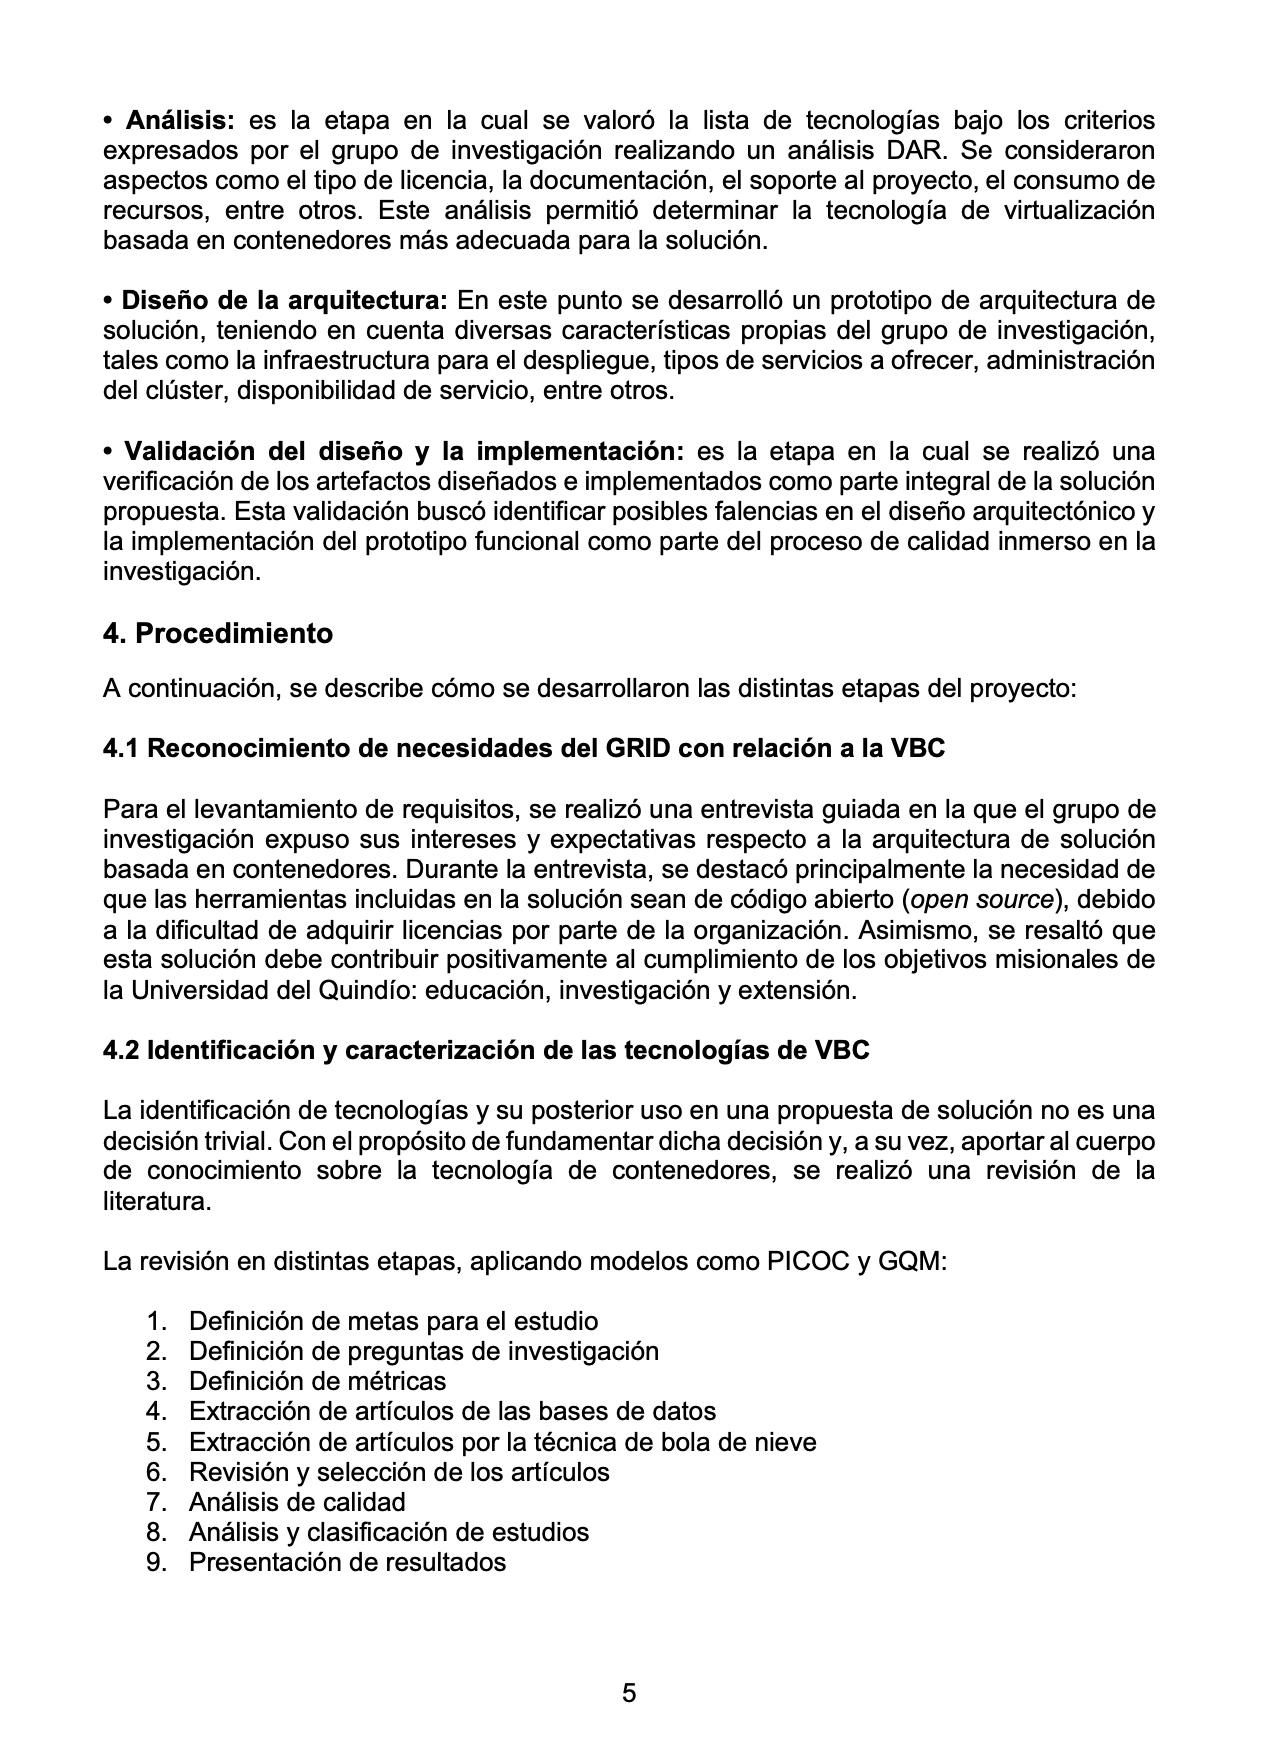
\includegraphics[width=0.95\textwidth,keepaspectratio]{apendices/ACOFI/pagina_7.png}
%	\end{tcolorbox}
%	\caption{Ponencia ACOFI --- Página 7}\label{fig:acofi-pagina-7}
%\end{figure}
%\FloatBarrier% Página 8
%\begin{figure}[H]
%	\centering
%	\begin{tcolorbox}[
%			colback=white,
%			colframe=gray!50,
%			boxrule=1pt,
%			arc=2pt,
%			boxsep=5pt,
%			left=3pt,
%			right=3pt,
%			top=3pt,
%			bottom=3pt,
%			drop shadow
%		]
%		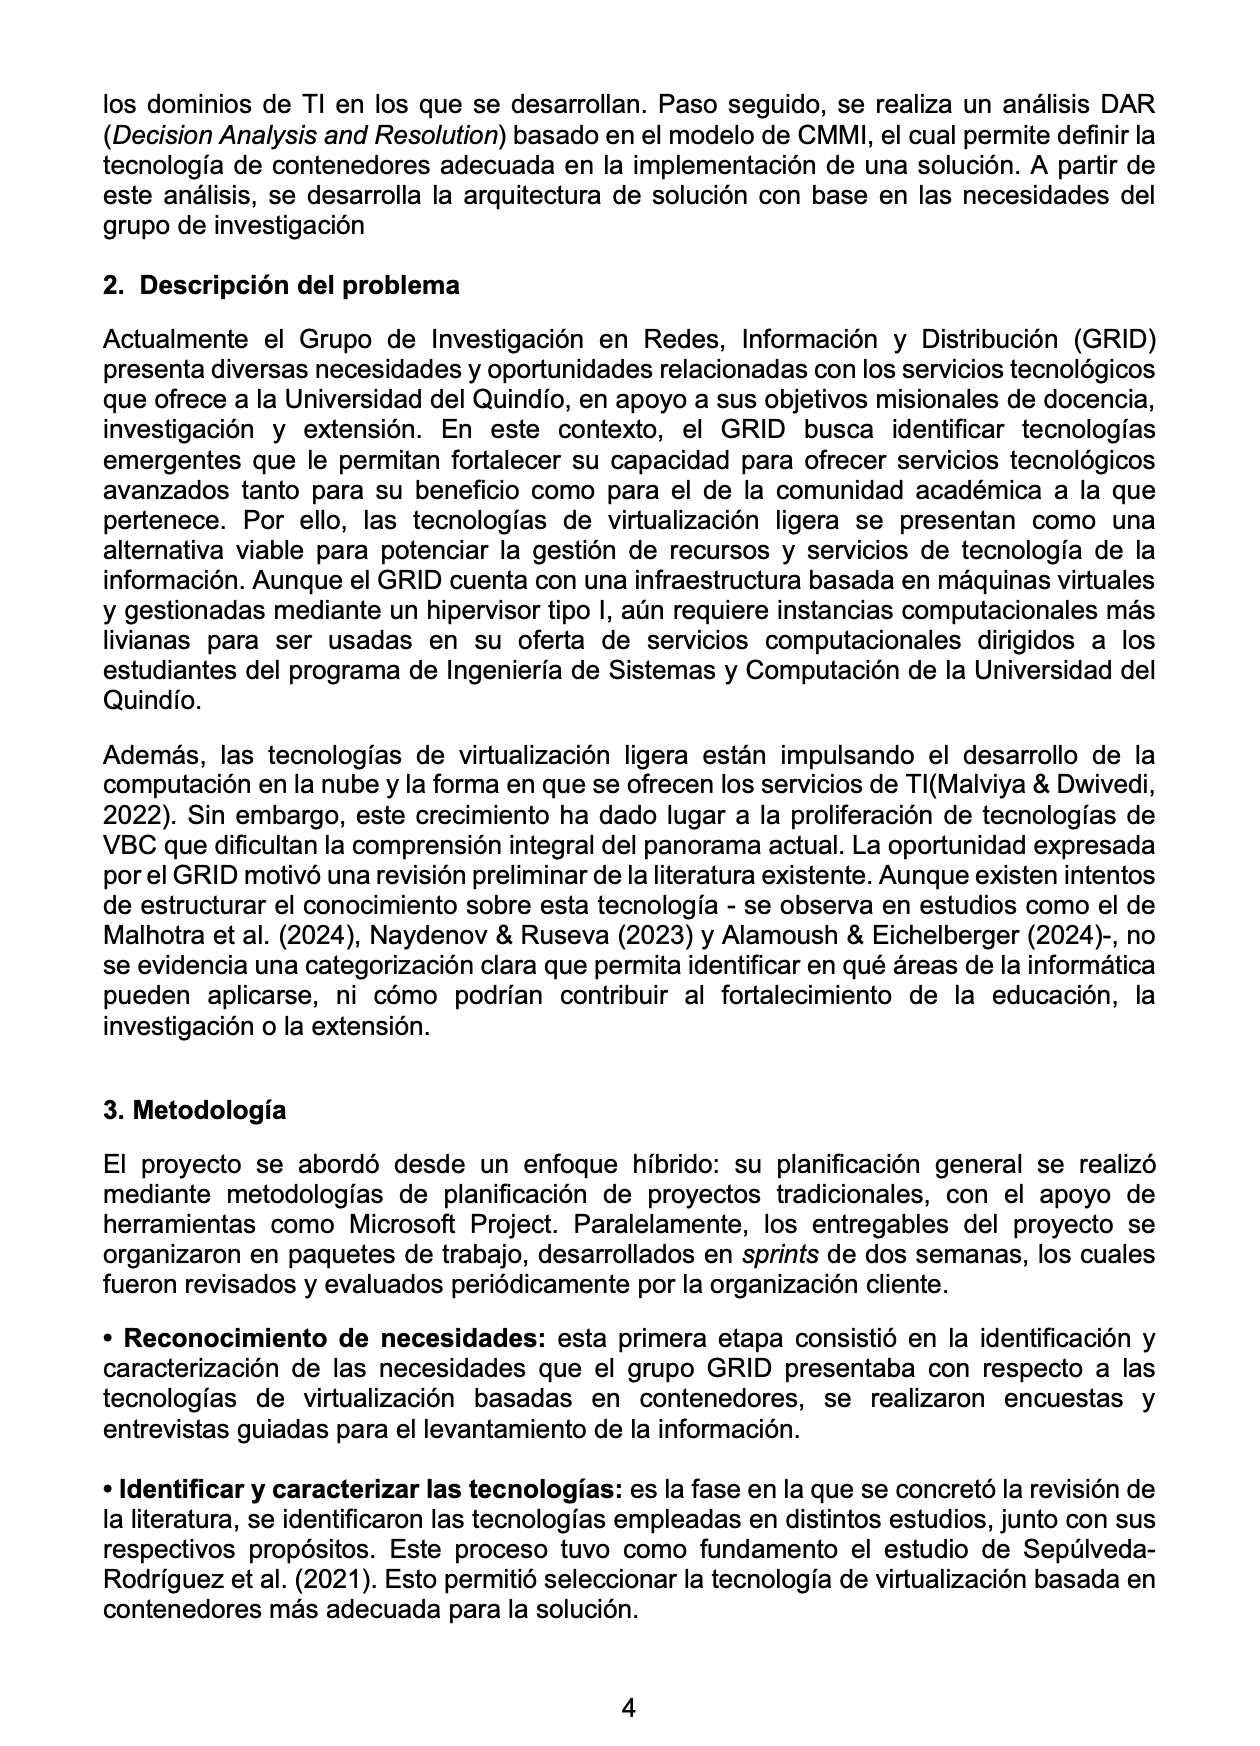
\includegraphics[width=0.95\textwidth,keepaspectratio]{apendices/ACOFI/pagina_8.png}
%	\end{tcolorbox}
%	\caption{Ponencia ACOFI --- Página 8}\label{fig:acofi-pagina-8}
%\end{figure}
%\FloatBarrier% Página 9
%\begin{figure}[H]
%	\centering
%	\begin{tcolorbox}[
%			colback=white,
%			colframe=gray!50,
%			boxrule=1pt,
%			arc=2pt,
%			boxsep=5pt,
%			left=3pt,
%			right=3pt,
%			top=3pt,
%			bottom=3pt,
%			drop shadow
%		]
%		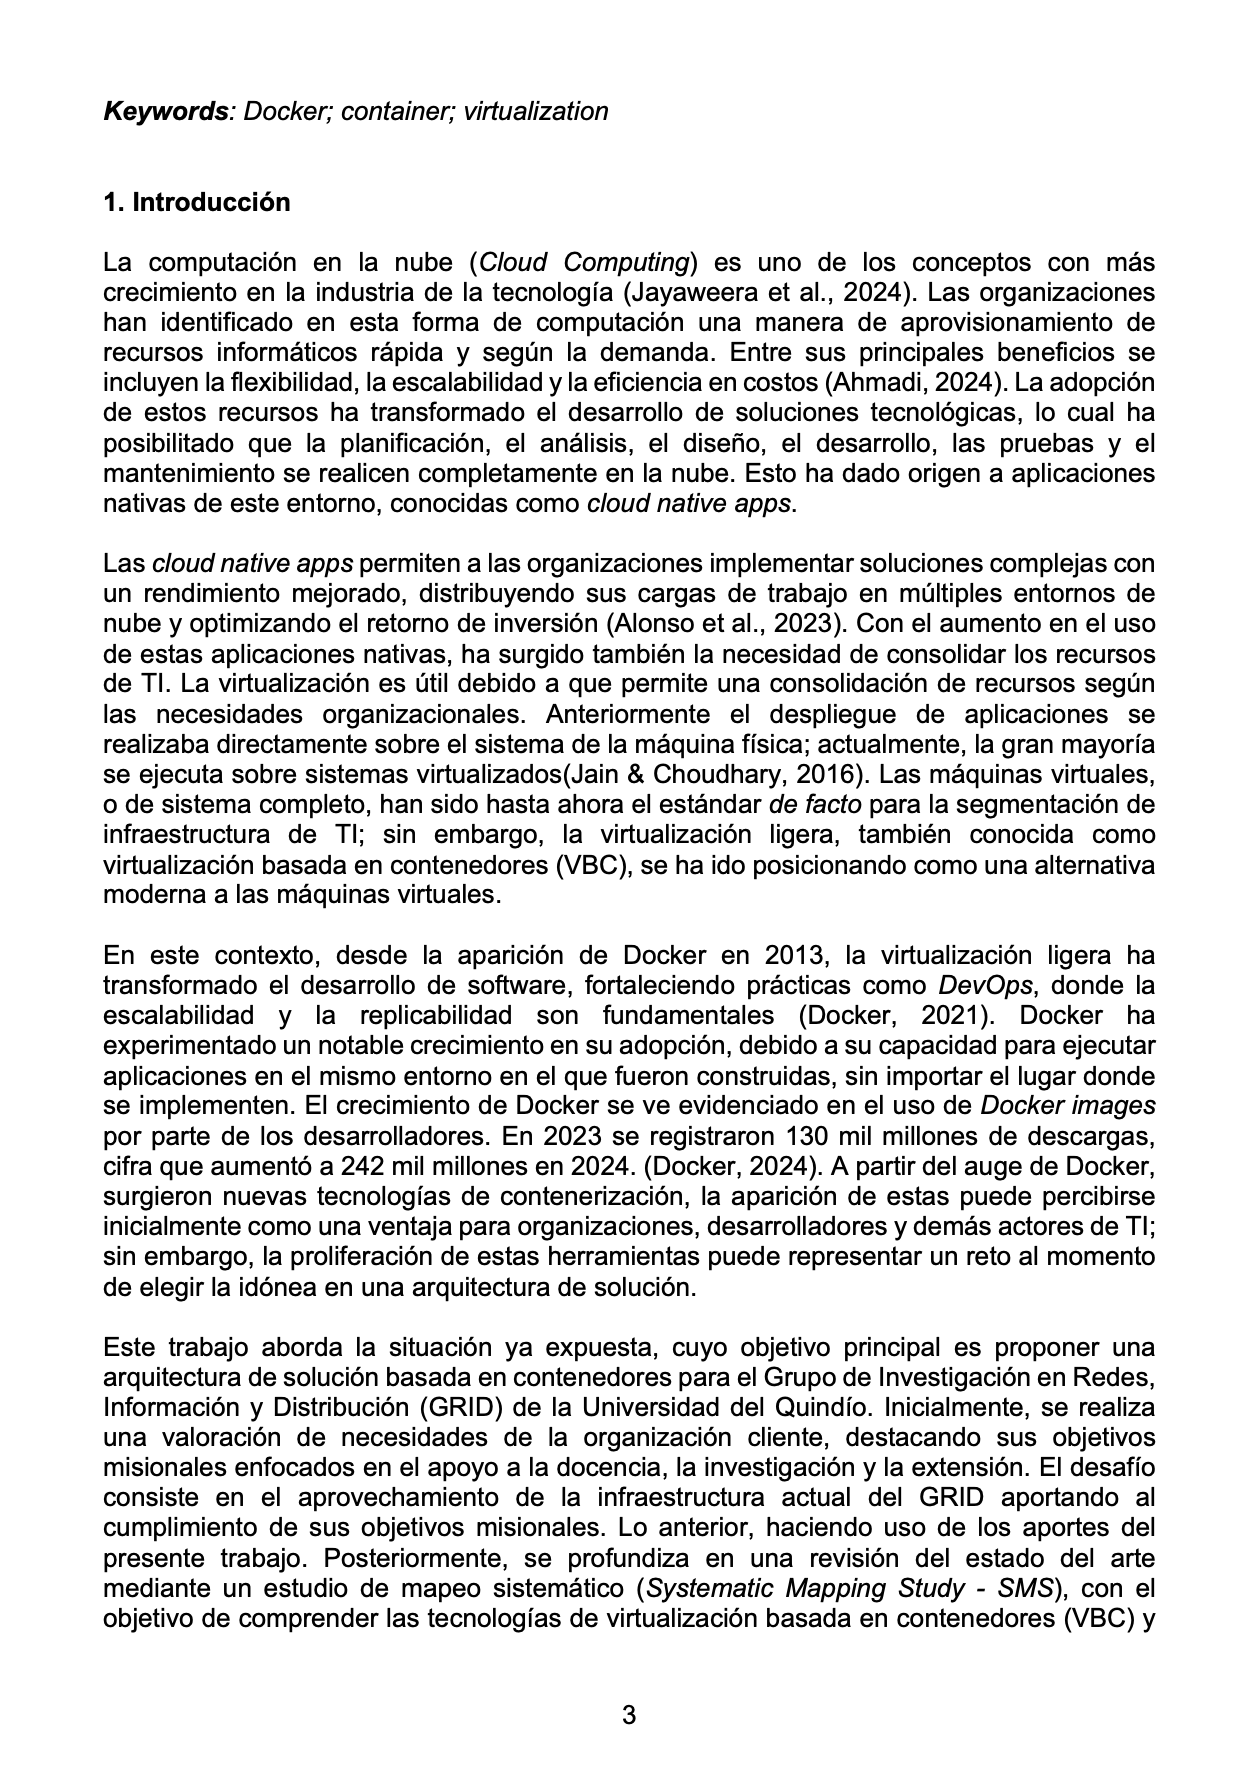
\includegraphics[width=0.95\textwidth,keepaspectratio]{apendices/ACOFI/pagina_9.png}
%	\end{tcolorbox}
%	\caption{Ponencia ACOFI --- Página 9}\label{fig:acofi-pagina-9}
%\end{figure}
%\FloatBarrier% Página 10
%\begin{figure}[H]
%	\centering
%	\begin{tcolorbox}[
%			colback=white,
%			colframe=gray!50,
%			boxrule=1pt,
%			arc=2pt,
%			boxsep=5pt,
%			left=3pt,
%			right=3pt,
%			top=3pt,
%			bottom=3pt,
%			drop shadow
%		]
%		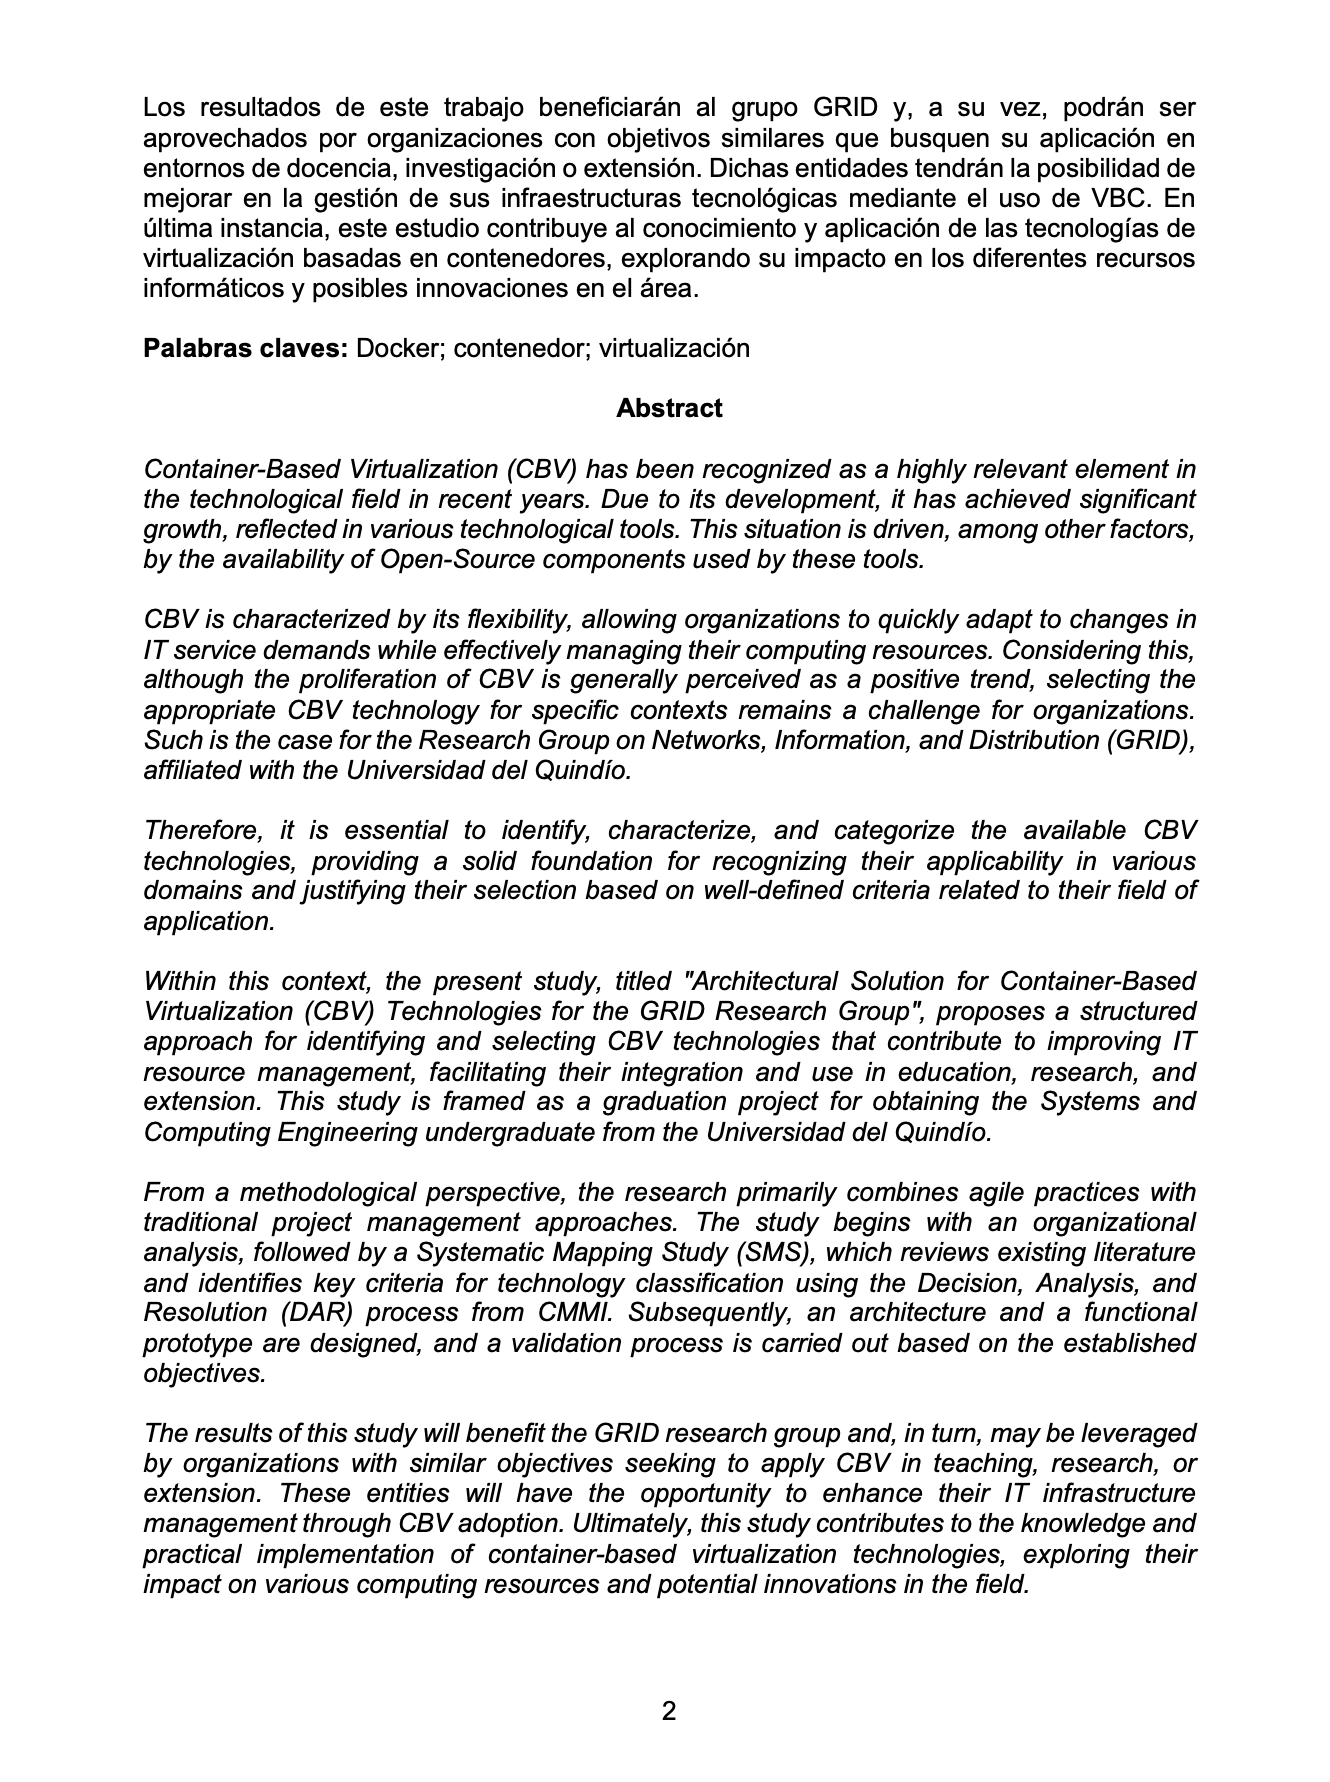
\includegraphics[width=0.95\textwidth,keepaspectratio]{apendices/ACOFI/pagina_10.png}
%	\end{tcolorbox}
%	\caption{Ponencia ACOFI --- Página 10}\label{fig:acofi-pagina-10}
%\end{figure}
%\FloatBarrier\section{CEIFI 2025}
%
%\section{Artículo de revista}
%
%En esta sección se presenta el artículo de revista publicado en Journal of Information Systems and Applications (JISA) como resultado de la investigación desarrollada en este trabajo.
%
%\subsection{Páginas del artículo JISA}
%
%% Página 1
%\begin{figure}[H]
%	\centering
%	\begin{tcolorbox}[
%			colback=white,
%			colframe=gray!50,
%			boxrule=1pt,
%			arc=2pt,
%			boxsep=5pt,
%			left=3pt,
%			right=3pt,
%			top=3pt,
%			bottom=3pt,
%			drop shadow
%		]
%		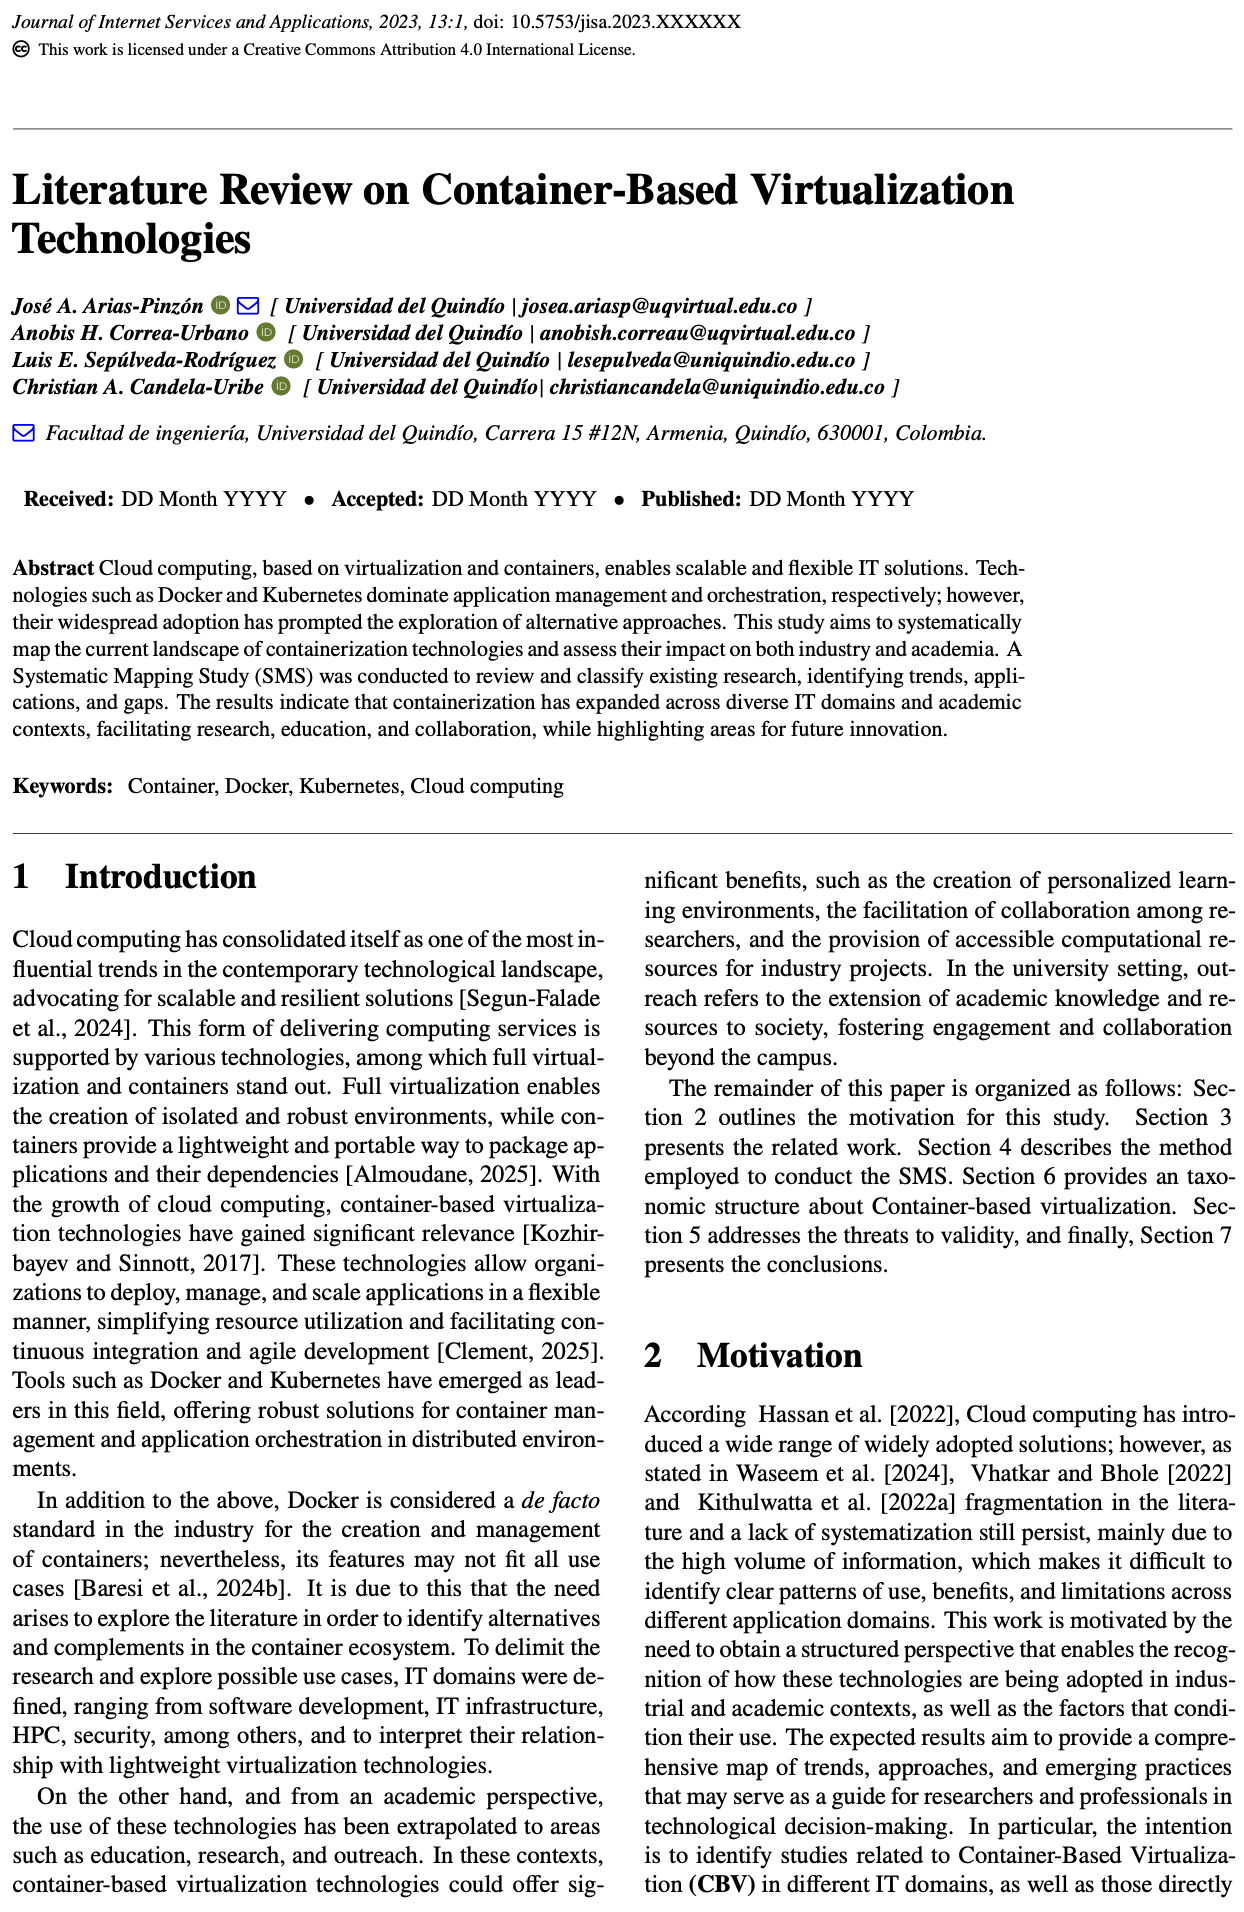
\includegraphics[width=0.95\textwidth,keepaspectratio]{apendices/JISA/pagina_1.png}
%	\end{tcolorbox}
%	\caption{Artículo JISA --- Página 1}\label{fig:jisa-pagina-1}
%\end{figure}
%\FloatBarrier% Página 2
%\begin{figure}[H]
%	\centering
%	\begin{tcolorbox}[
%			colback=white,
%			colframe=gray!50,
%			boxrule=1pt,
%			arc=2pt,
%			boxsep=5pt,
%			left=3pt,
%			right=3pt,
%			top=3pt,
%			bottom=3pt,
%			drop shadow
%		]
%		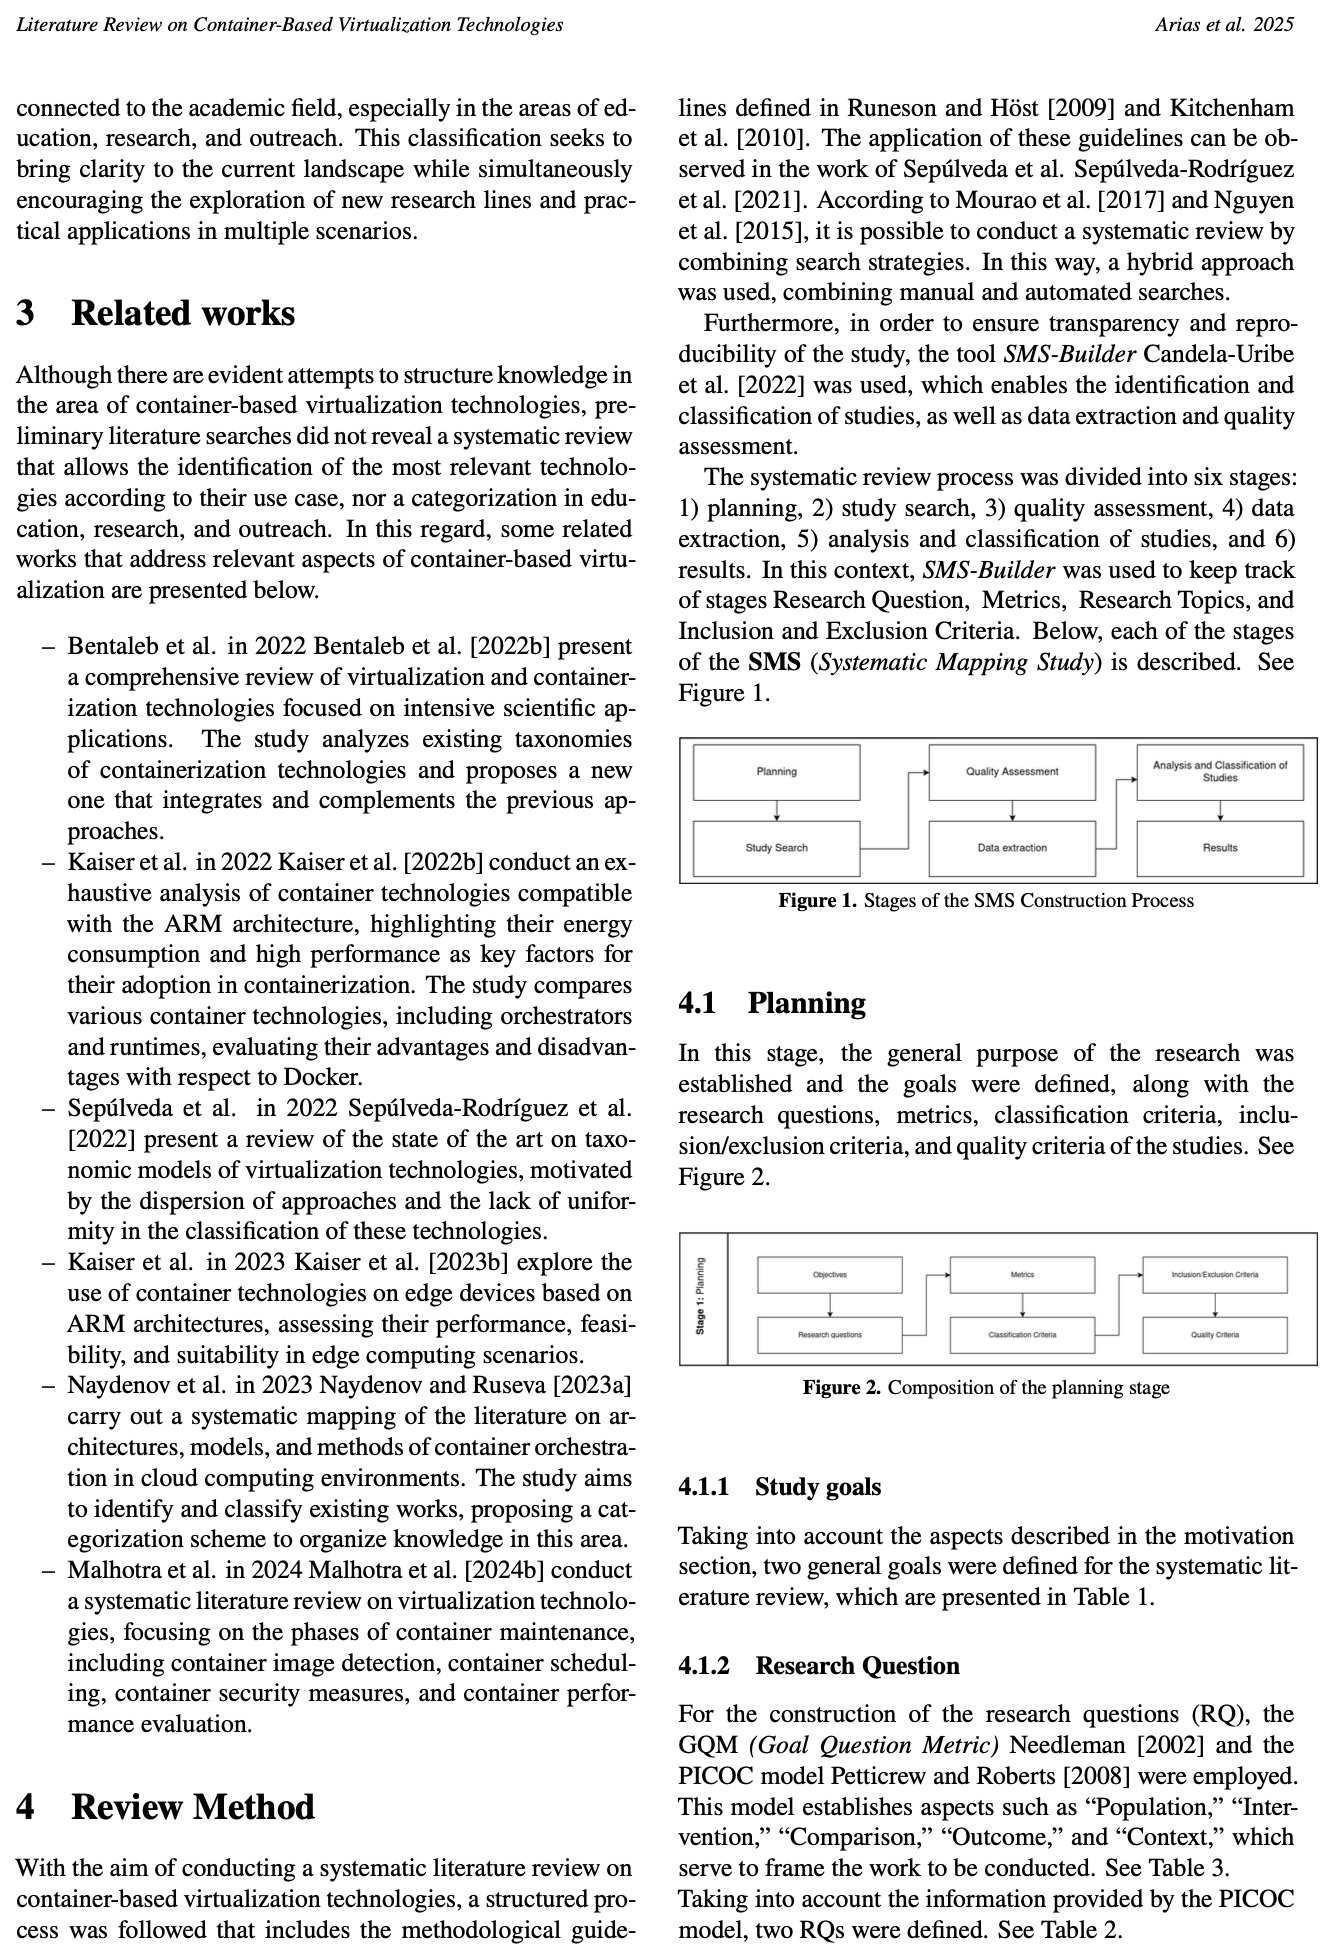
\includegraphics[width=0.95\textwidth,keepaspectratio]{apendices/JISA/pagina_2.png}
%	\end{tcolorbox}
%	\caption{Artículo JISA --- Página 2}\label{fig:jisa-pagina-2}
%\end{figure}
%\FloatBarrier% Página 3
%\begin{figure}[H]
%	\centering
%	\begin{tcolorbox}[
%			colback=white,
%			colframe=gray!50,
%			boxrule=1pt,
%			arc=2pt,
%			boxsep=5pt,
%			left=3pt,
%			right=3pt,
%			top=3pt,
%			bottom=3pt,
%			drop shadow
%		]
%		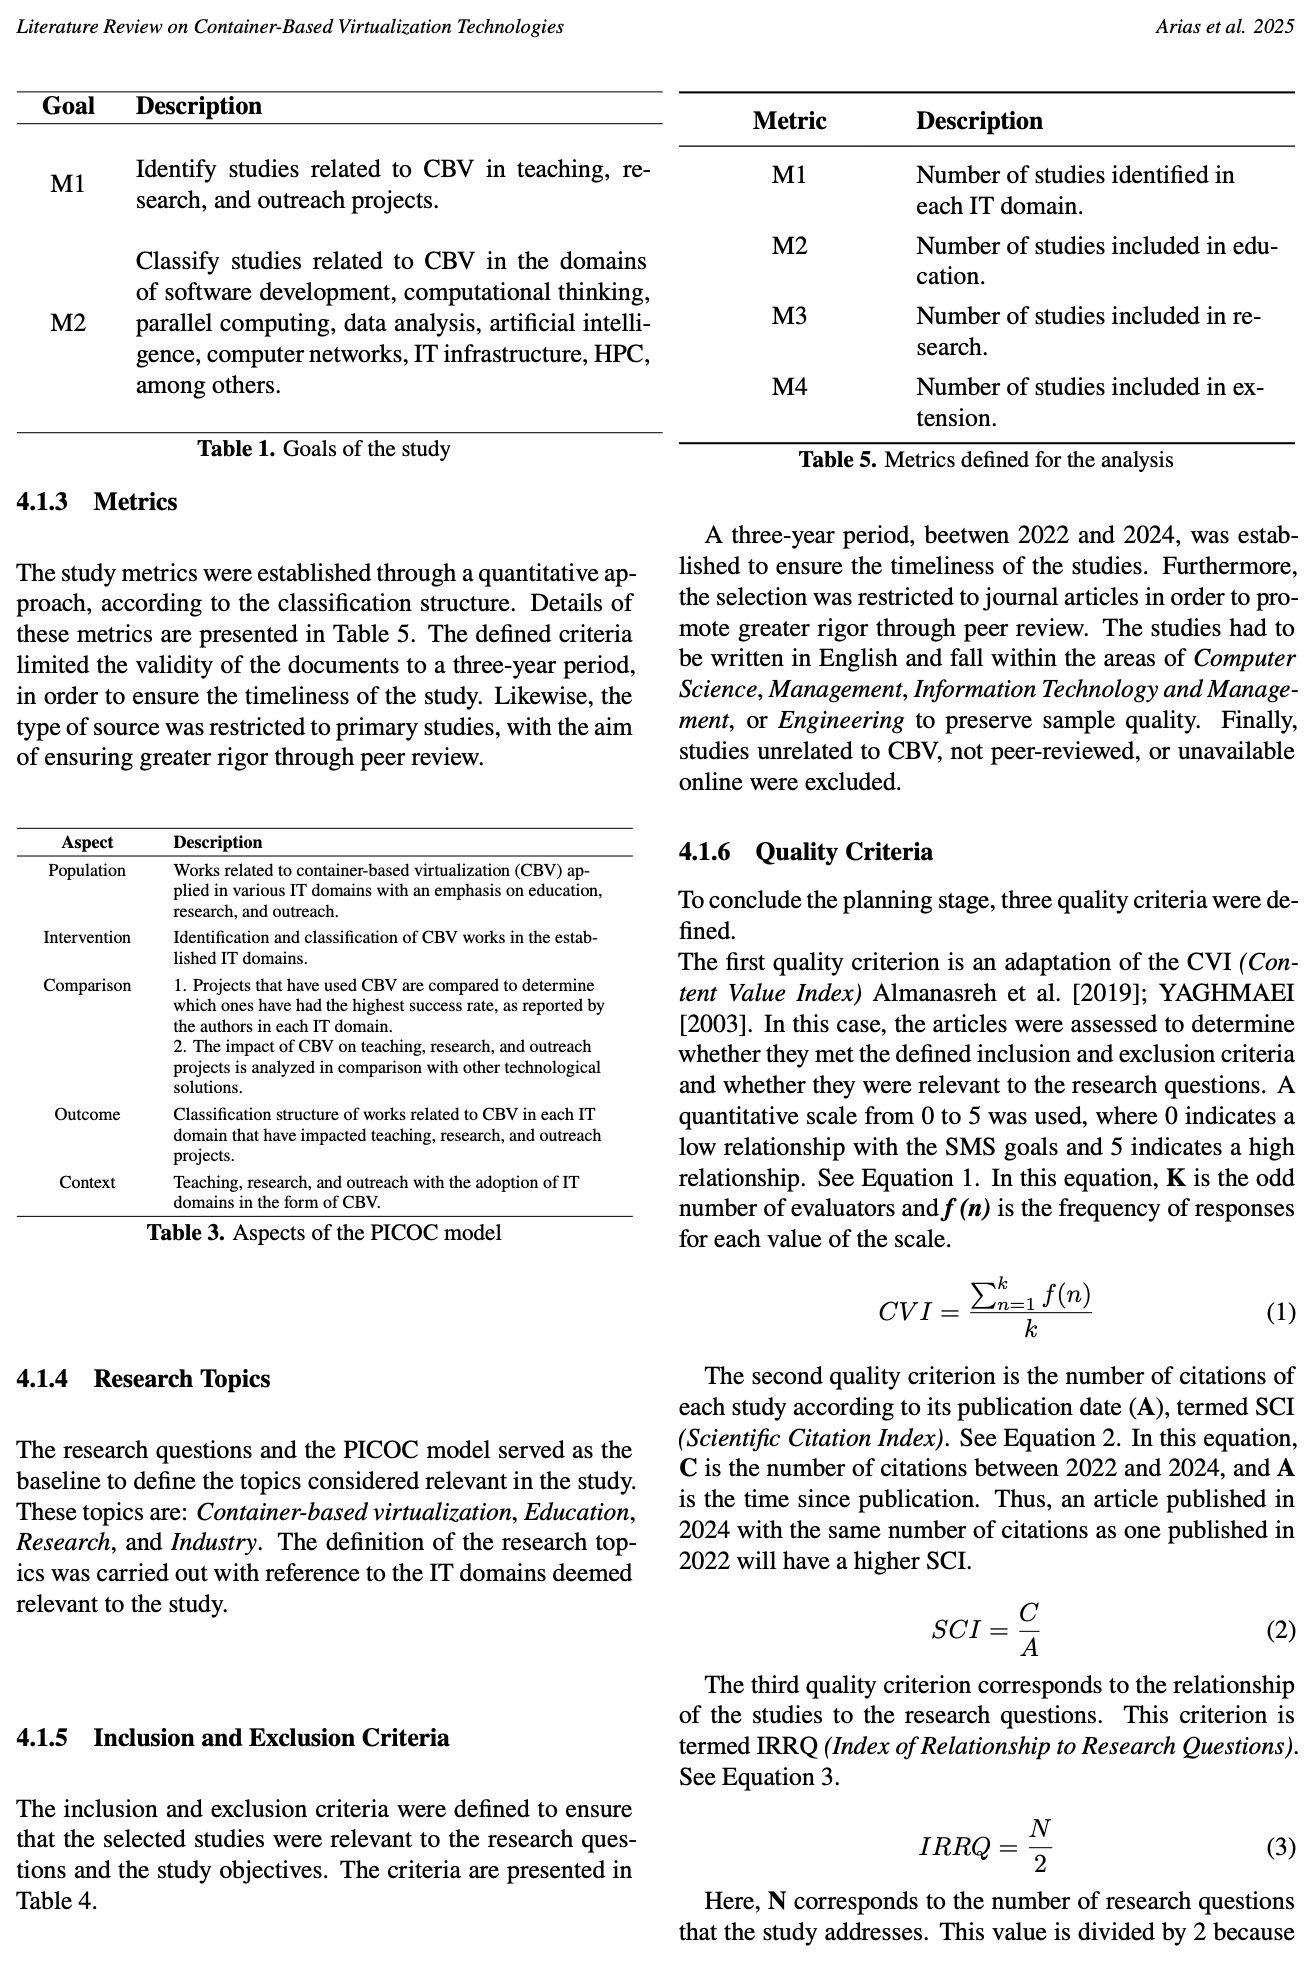
\includegraphics[width=0.95\textwidth,keepaspectratio]{apendices/JISA/pagina_3.png}
%	\end{tcolorbox}
%	\caption{Artículo JISA --- Página 3}\label{fig:jisa-pagina-3}
%\end{figure}
%\FloatBarrier% Página 4
%\begin{figure}[H]
%	\centering
%	\begin{tcolorbox}[
%			colback=white,
%			colframe=gray!50,
%			boxrule=1pt,
%			arc=2pt,
%			boxsep=5pt,
%			left=3pt,
%			right=3pt,
%			top=3pt,
%			bottom=3pt,
%			drop shadow
%		]
%		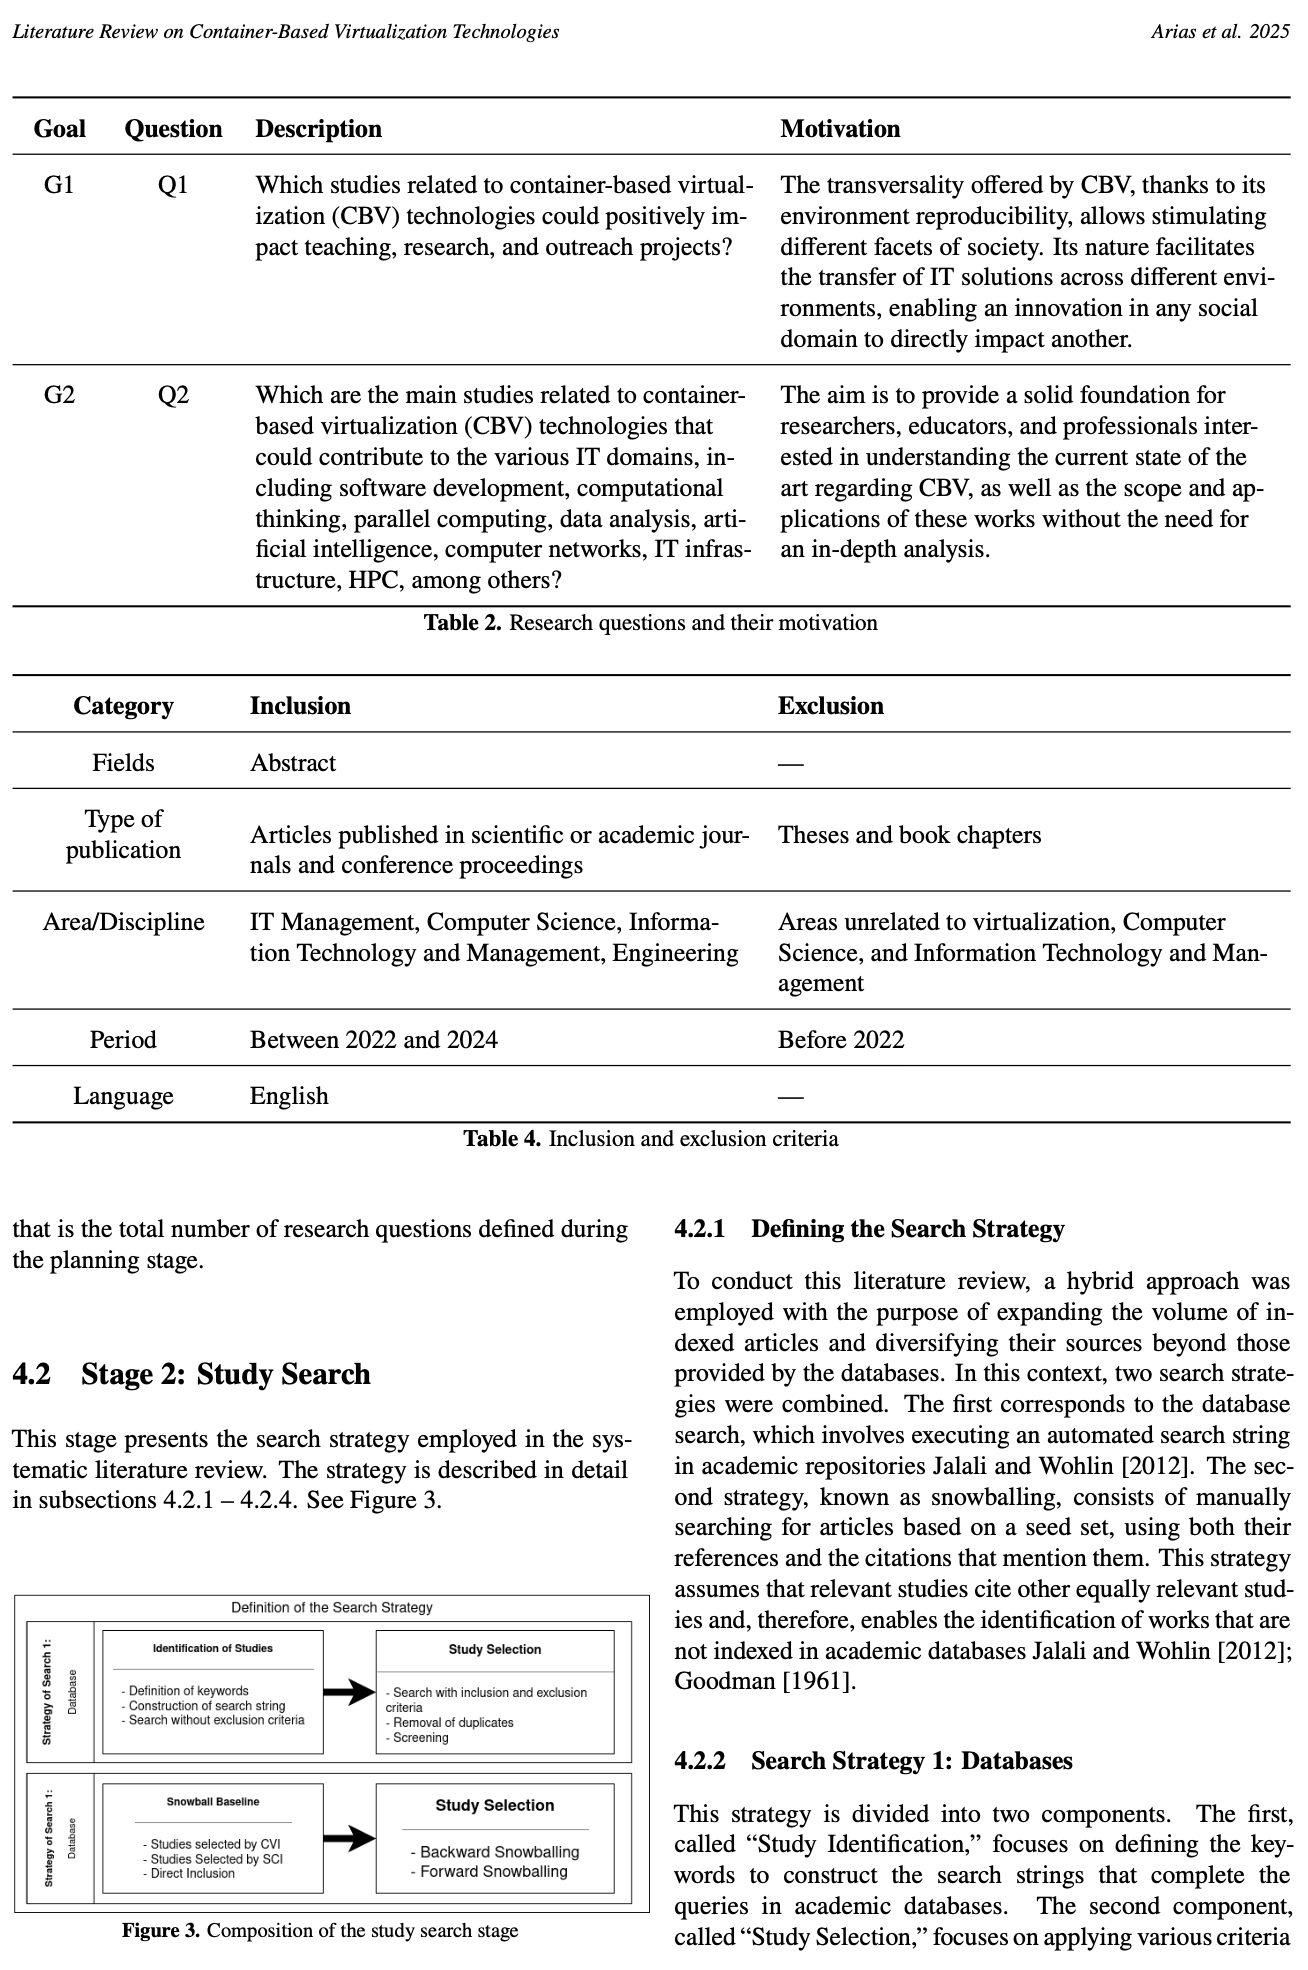
\includegraphics[width=0.95\textwidth,keepaspectratio]{apendices/JISA/pagina_4.png}
%	\end{tcolorbox}
%	\caption{Artículo JISA --- Página 4}\label{fig:jisa-pagina-4}
%\end{figure}
%\FloatBarrier% Página 5
%\begin{figure}[H]
%	\centering
%	\begin{tcolorbox}[
%			colback=white,
%			colframe=gray!50,
%			boxrule=1pt,
%			arc=2pt,
%			boxsep=5pt,
%			left=3pt,
%			right=3pt,
%			top=3pt,
%			bottom=3pt,
%			drop shadow
%		]
%		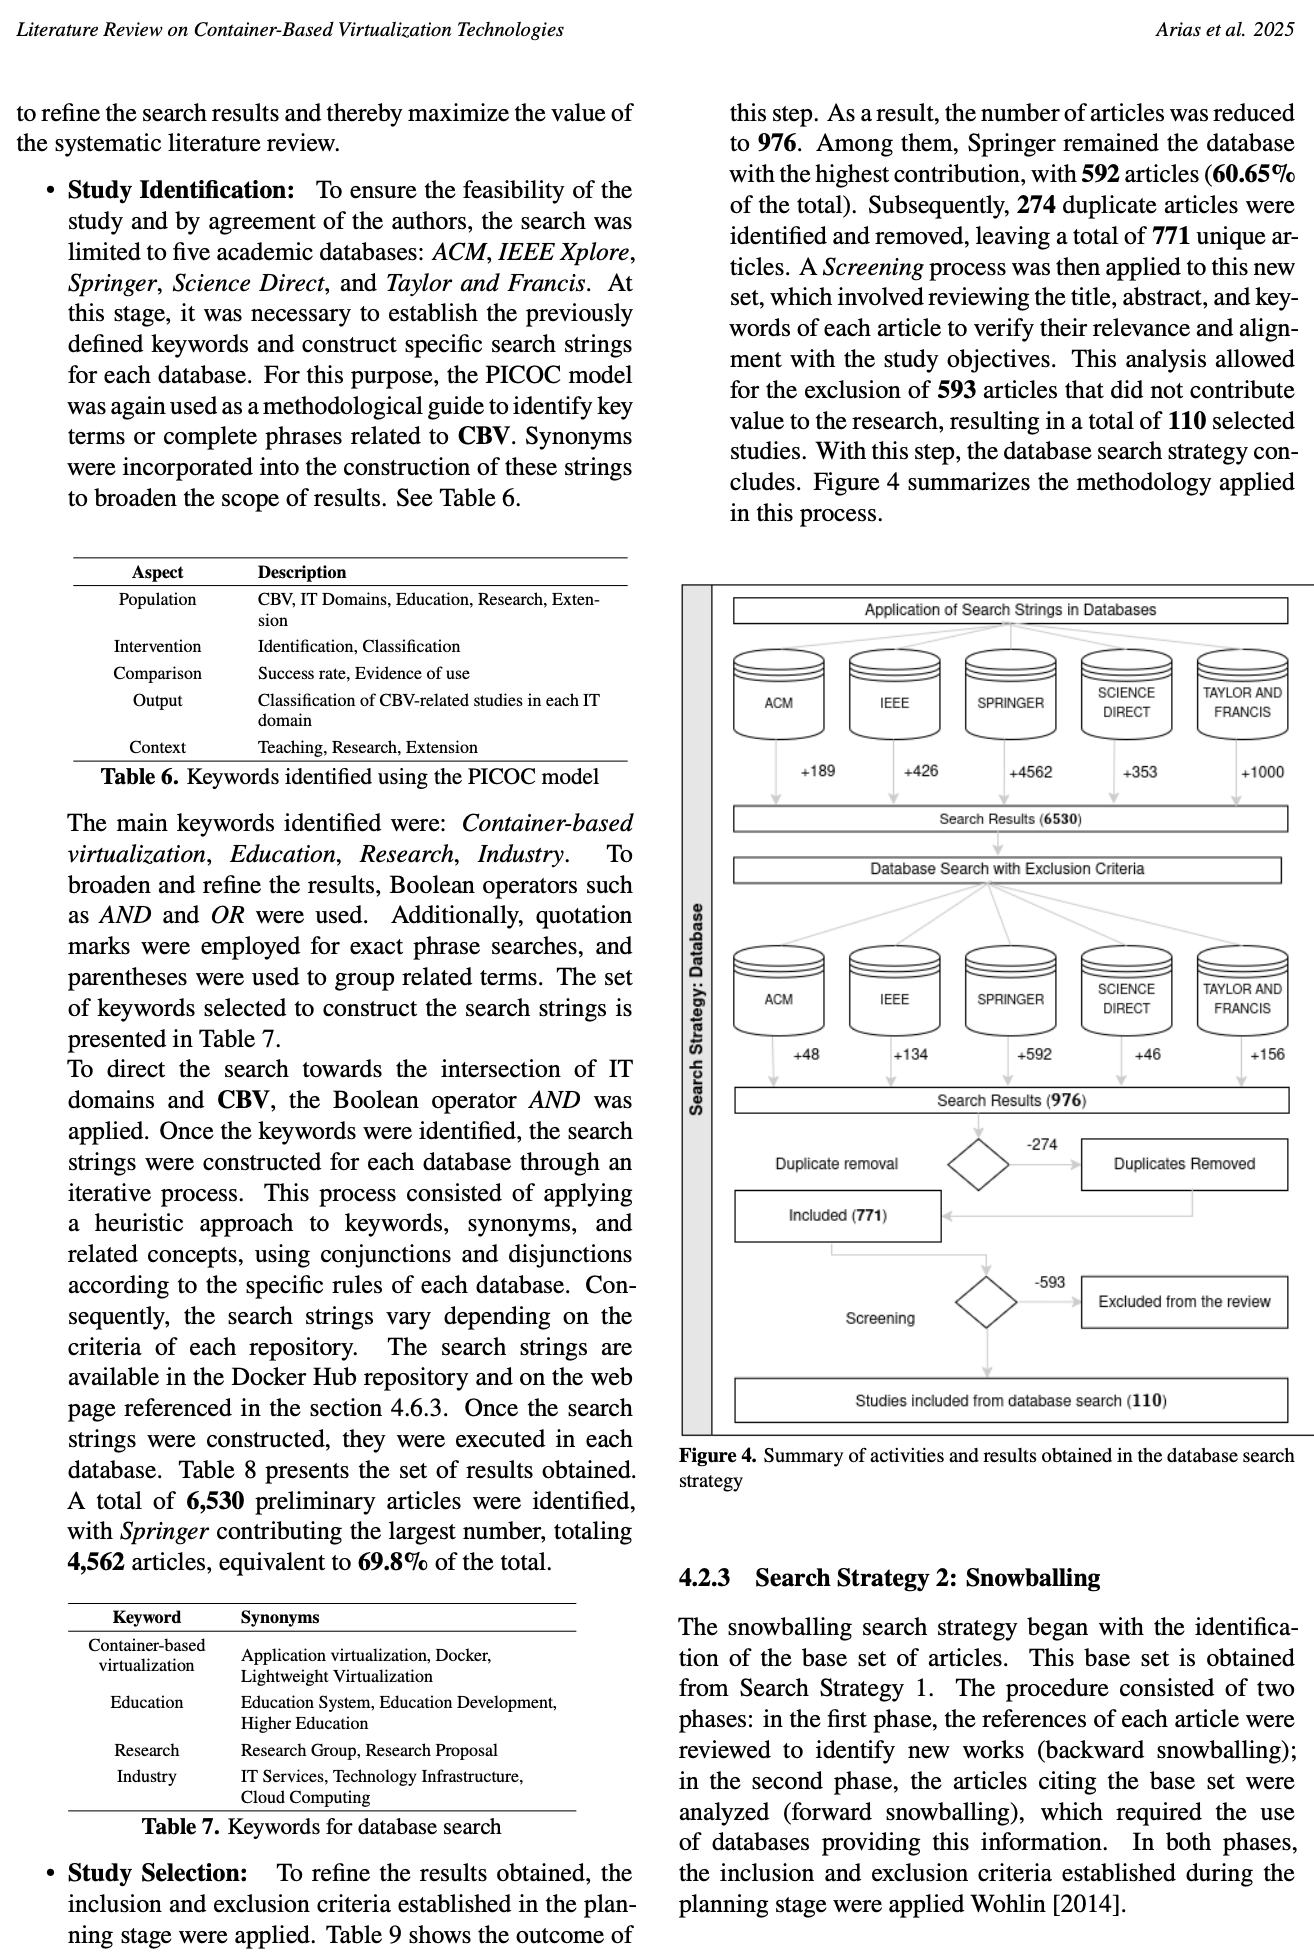
\includegraphics[width=0.95\textwidth,keepaspectratio]{apendices/JISA/pagina_5.png}
%	\end{tcolorbox}
%	\caption{Artículo JISA --- Página 5}\label{fig:jisa-pagina-5}
%\end{figure}
%\FloatBarrier% Macro para crear páginas del artículo de forma automática
%% Páginas 6-34
%\newcounter{jisampage}
%\setcounter{jisampage}{6}
%\loop%
%\begin{figure}[H]
%	\centering
%	\begin{tcolorbox}[
%			colback=white,
%			colframe=gray!50,
%			boxrule=1pt,
%			arc=2pt,
%			boxsep=5pt,
%			left=3pt,
%			right=3pt,
%			top=3pt,
%			bottom=3pt,
%			drop shadow
%		]
%		\includegraphics[width=0.95\textwidth,keepaspectratio]{apendices/JISA/pagina_\thejisampage.png}
%	\end{tcolorbox}
%	\caption{Artículo JISA --- Página \thejisampage}\label{fig:jisa-pagina-\thejisampage}
%\end{figure}
%\FloatBarrier\stepcounter{jisampage}
%\ifnum\value{jisampage}<35
%\repeat%
%
%\section{Slides de CEIFI}
%\foreach \n in {1,...,16} {
%		\begin{figure}[H]
%			\centering
%			\fbox{\includegraphics[width=0.9\textwidth]{apendices/CEIFI/\n.png}}
%			\caption{Slide \n de CEIFI}
%		\end{figure}
%	}
%
%\section{Slides de GRID 2025-I}
%\foreach \n in {1,...,13} {
%		\begin{figure}[H]
%			\centering
%			\fbox{\includegraphics[width=0.9\textwidth]{apendices/GRID-2025/\n.png}}
%			\caption{Slide \n de GRID 2025-I}
%		\end{figure}
%	}
%
%\section{Poster GRID 2024-II}
%\begin{figure}[H]
%	\centering
%	\fbox{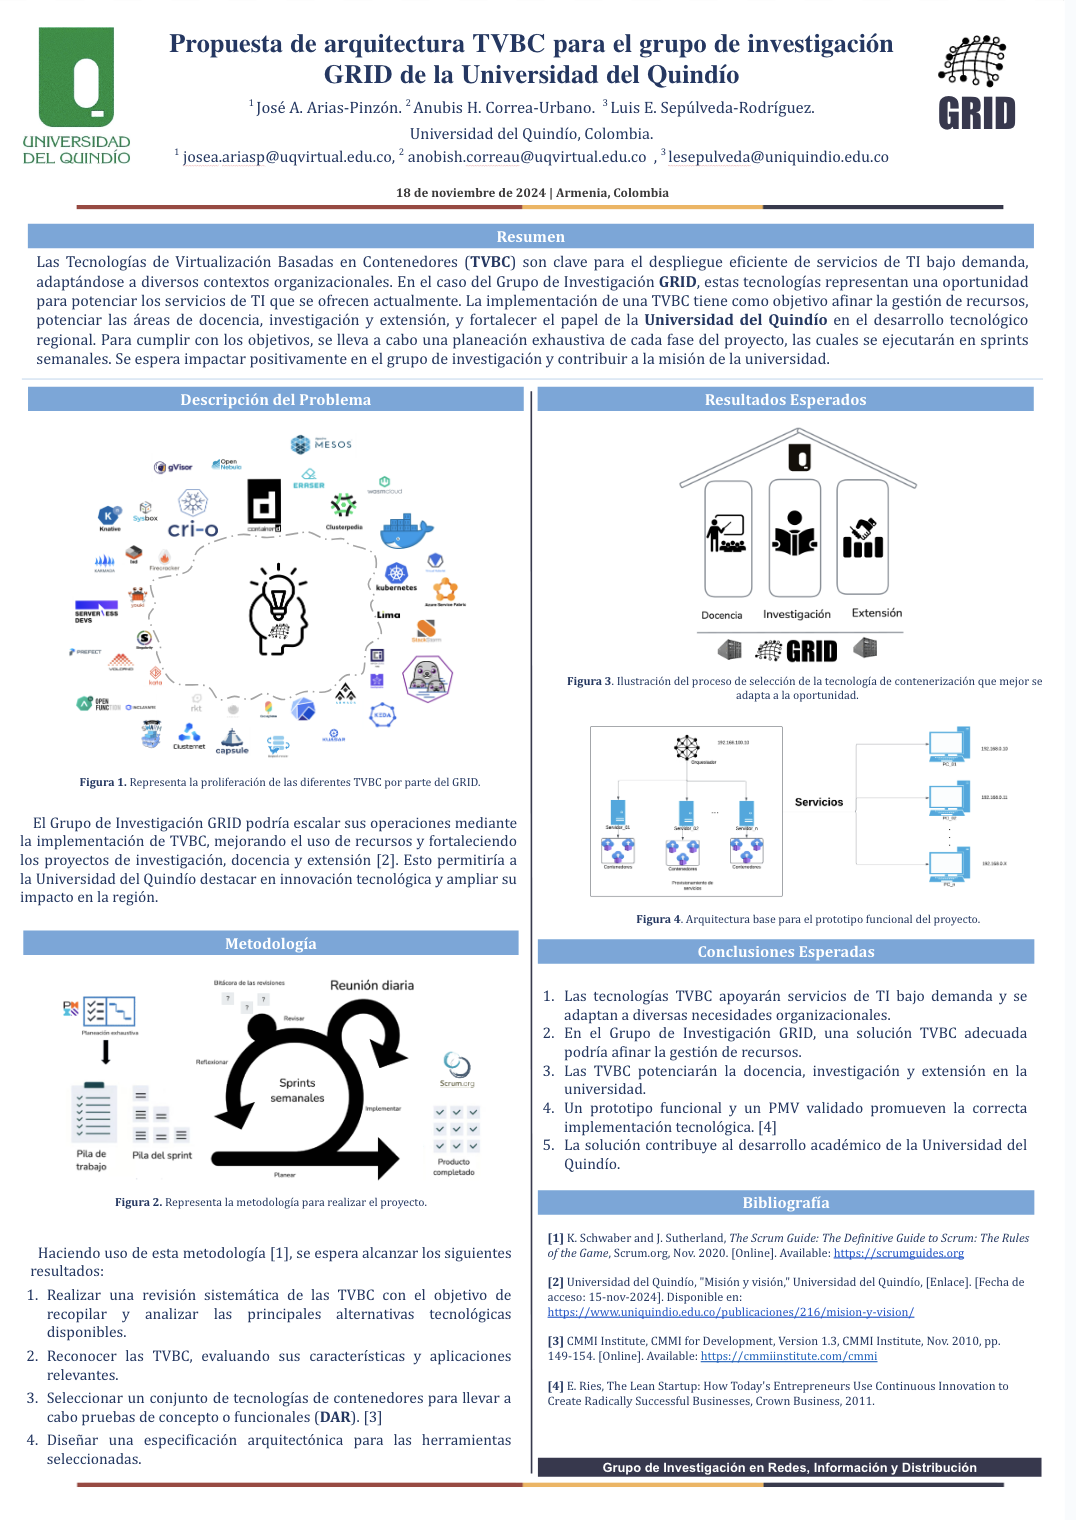
\includegraphics[width=0.9\textwidth]{apendices/GRID-2024/image.png}}
%	\caption{Póster de GRID 2024-II}
%\end{figure}
